\documentclass[conference]{IEEEtran}
\IEEEoverridecommandlockouts
% The preceding line is only needed to identify funding in the first footnote. If that is unneeded, please comment it out.
\usepackage{cite}
\usepackage{amsmath,amssymb,amsfonts}
\usepackage{algorithmic}
\usepackage{graphicx}
\usepackage{textcomp}
\usepackage{xcolor}
\usepackage[utf8]{inputenc} % allow utf-8 input
\usepackage[T1]{fontenc}    % use 8-bit T1 fonts
\usepackage{hyperref}       % hyperlinks
\usepackage{url}            % simple URL typesetting
\usepackage{booktabs}       % professional-quality tables
\usepackage{amsfonts}       % blackboard math symbols
\usepackage{nicefrac}       % compact symbols for 1/2, etc.
\usepackage{microtype}      % microtypography
\usepackage{lipsum}         % Can be removed after putting your text content
\usepackage{graphicx}
\usepackage{natbib}
\usepackage{doi}
\usepackage{svg}
\usepackage{amsmath}
\usepackage{multirow}
\usepackage{adjustbox}
\usepackage{subcaption}
\usepackage{appendix}
\usepackage{verbatim}
\usepackage{CJK}
\usepackage{minted}
\usepackage{fvextra}
\usepackage[table,xcdraw]{xcolor}
\usepackage{threeparttable} 
\def\BibTeX{{\rm B\kern-.05em{\sc i\kern-.025em b}\kern-.08em
    T\kern-.1667em\lower.7ex\hbox{E}\kern-.125emX}}

\usepackage{listings}
\usepackage{color}
\usepackage{subfig}

\definecolor{mygreen}{rgb}{0,0.6,0}
\definecolor{mygray}{rgb}{0.5,0.5,0.5}
\definecolor{mymauve}{rgb}{0.58,0,0.82}
\definecolor{lightgray}{rgb}{0.95,0.95,0.95}

\lstset{ %
  backgroundcolor=\color{lightgray},   % choose the background color; you must add \usepackage{color} or \usepackage{xcolor}; should come as last argument
  basicstyle=\footnotesize\ttfamily,        % the size of the fonts that are used for the code
  breakatwhitespace=false,         % sets if automatic breaks should only happen at whitespace
  breaklines=true,                 % sets automatic line breaking
  captionpos=b,                    % sets the caption-position to bottom
  commentstyle=\color{mygreen},    % comment style
  escapeinside={\%*}{*)},          % if you want to add LaTeX within your code
  keywordstyle=\color{blue},       % keyword style
  stringstyle=\color{mymauve},     % string literal style
}
    % define AIbox
\usepackage[most]{tcolorbox}
\usepackage{float}
\usepackage{xspace}
\tcbset{
  aibox/.style={
    width=\textwidth,
    top=10pt,
    colback=white,
    colframe=black,
    colbacktitle=black,
    enhanced,
    center,
    attach boxed title to top left={yshift=-0.1in,xshift=0.15in},
    boxed title style={boxrule=0pt,colframe=white,},
  }
}
\newtcolorbox{AIbox}[2][]{aibox,title=#2,#1}


\tcbset{
  aibox1/.style={
    width=\columnwidth, % 适应IEEE单栏宽度
    top=10pt,
    colback=white, % 内部背景颜色
    colframe=black, % 边框颜色
    colbacktitle=black, % 标题背景颜色
    enhanced,
    center,
    attach boxed title to top left={yshift=-0.1in, xshift=0.15in}, % 标题位置调整
    boxed title style={boxrule=0pt, colframe=white}, % 标题框样式
  }
}

% 根据aibox样式定义新的AIbox1环境
\newtcolorbox{AIbox1}[2][]{aibox1,title=#2,#1}

\DefineVerbatimEnvironment{Verbatim}{Verbatim}{
  fontsize=\fontsize{8pt}{9.5pt}\selectfont, % 设置字体大小为9pt,行间距为11pt
  breaklines=true  % 允许自动换行
}

\title{Travel Insurance Recommendation AI System Based on Flight Delay Predictions and Customer Sentiment}


\author{
    \IEEEauthorblockN{
        Yuzhe Yang\IEEEauthorrefmark{1},
        Haoqi Zhang\IEEEauthorrefmark{1},
        Zhidong Peng\IEEEauthorrefmark{1},
        Yilin Guo\IEEEauthorrefmark{2},
        Tianji Zhou\IEEEauthorrefmark{3}
    }
    \IEEEauthorblockA{\{121090684, 121090766, 121090448, 121020064, 121090858\}@link.cuhk.edu.cn} %按名字写自己学号
    \IEEEauthorblockA{\IEEEauthorrefmark{1}School of Data Science}
    \IEEEauthorblockA{\IEEEauthorrefmark{2}School of Medicine}
    \IEEEauthorblockA{\IEEEauthorrefmark{3}School of Management and Economics}
}




\begin{document}
\pagestyle{plain}
\maketitle

\begin{abstract}

\textbf{In this project, we designed an AI system to identify potential travel insurance intentions of customers. Our designed large language model (LLM), named Insurance-GPT, is capable of analyzing in real-time during interactions with users and it utilizes deep learning model to accurately predict flight delay. This provides a good user experience, as well as provides a reference for pricing strategies to insurance companies. The Insurance-GPT can be downloaded at \url{https://modelscope.cn/models/TobyYang7/InsuranceGPT}. Additionally, the complete source code for this project is available on GitHub at \url{https://github.com/TobyYang7/Travel-Insurance-Recommendation-AI-System}.}

\end{abstract}


\begin{IEEEkeywords}
Large Language Model, Graph Convolutional Networks, Spatio-Temporal Data Mining
\end{IEEEkeywords}

\section{Introduction}

As the global economy and aviation industry develops, more people choose to travel by plane for both leisure and business purposes. However, there is a significant challenge that has come along with this growth: flight delays. According to a 2023 report, approximately 20.37\% of flights in the U.S. were delayed by 15 minutes or more, causing a ripple effect of inconveniences for passengers, such as disrupted travel plans, and leading to considerable economic impacts for airlines \cite{bureau2023airline}.  The Federal Aviation Administration (FAA) estimated the annual cost of these delays to be around \$33 billion in 2019 \cite{faa2020}. In response to this prevalent issue, flight delay insurance has arisen, providing financial protection against unexpected delays. This insurance, either sold as a standalone policy or as a supplementary coverage to travel accident insurance, underwrites the airline's on-time departure credibility and compensates passengers for delays-related inconveniences. However, the way that currently prices this insurance is impersonal, failing to account for individual passengers' preferences, which easily results in a low buying rate and potential dissatisfaction. Furthermore, many airlines rely on average values based on historical records for delay predictions, underscoring an urgent need for more accurate flight delay prediction. 

This project presents a novel AI system designed to predict flight delays and price insurance accordingly, enabling airlines to provide personalized insurance recommendations for passengers. The proposed system analyzes flight delay rates based on multiple relevant data sources, including flight dynamics, city weather, and special situation data. Additionally, it constructs user profiles via sentiment analysis of customer feedback to airlines, offering tailored and optimal insurance recommendations to improve insurance purchase rates.

The primary objective of this system is to provide a tailored service for each customer, thereby enhancing customer satisfaction and loyalty and also increasing airline revenue. With its emphasis on prediction accuracy and user interaction quality, the AI system has the potential to reshape customer service in the airline industry, offering a competitive edge for airlines and promoting a positive brand image. Besides, from a long-term perspective, significant cost savings through automation of administrative tasks, enhanced income via dynamic and personalized pricing, and improved risk management facilitated by AI predictions are notable benefits.

\section{Framework}

\begin{figure}[h]
    \centering
    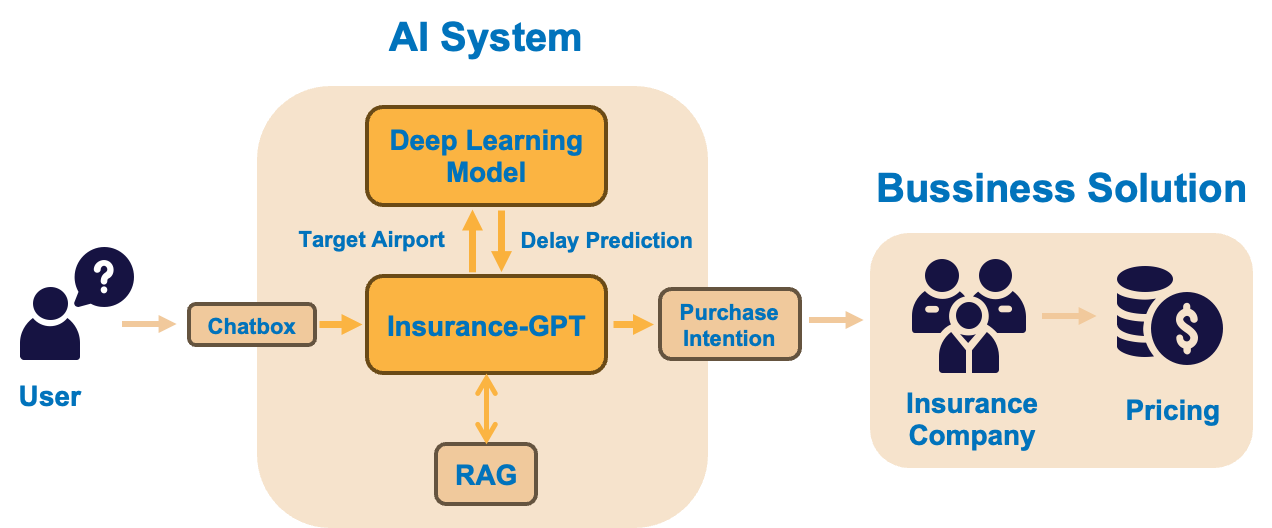
\includegraphics[width=1\linewidth]{image.png}
    \caption{AI-driven Framework}
    \label{fig:Framework}
\end{figure}

As shown in Fig. \ref{fig:Framework}, in the proposed scenario, users engage with the AI system through a chat interface. Then AI will utilize the deep learning model to predict airport delays based on the user's query. Once the AI has predicted possible airport delays, it proceeds to analyze the gathered data to infer the potential purchase intentions of the users. This step is crucial as it allows the insurance company to adapt its pricing strategy dynamically. By understanding and anticipating user needs based on predictive analysis, the company can offer tailored insurance solutions that cater to the specific circumstances of each customer.

The application of this AI-driven framework ensures a more personalized and responsive approach to customer service, enhancing the user experience and improving operational efficiency for the insurance company. The whole process not only contributes to higher customer satisfaction but also drives better financial performance through customized offerings.


\section{Data Engineering}

\subsection{Large Language Model Datasets}

\subsubsection{Datasets Overview}

To rigorously evaluate the performance of LLMs in the insurance sector, we meticulously selected three pivotal datasets, each offering unique insights and challenges:

\begin{itemize}
    \item \textbf{Travel Insurance Dataset \footnote{\url{https://www.kaggle.com/datasets/marwandiab/travel-insurance-dataset}}}: This dataset is crucial for understanding customer behavior related to travel insurance purchases. It includes comprehensive customer profiles, detailing features such as age, employment type, graduate status, annual income, family members, chronic diseases, frequent flyer status, and international travel history. Each profile is assessed and classified into categories labeled as either 'positive' or 'negative' based on their potential to purchase insurance. These features allow the LLM to predict purchasing tendencies effectively. To enhance our model's ability to generalize and interpret nuanced human sentiments, we have reclassified the original binary labels into four categories—negative, very negative, positive, and very positive—using GPT-3.5. This modification aims to refine our model's sensitivity to varying degrees of sentiment, which is critical for applications in customer service and targeted marketing.

    \item \textbf{Twitter US Airline Sentiment \footnote{\url{https://www.kaggle.com/datasets/crowdflower/twitter-airline-sentiment?resource=download&select=Tweets.csv}}}: This dataset is selected for its real-world applicability and consists of user-generated reviews about US airlines, categorized as positive or negative. The dataset provides a rich source for analyzing sentiment, which is crucial for training our LLM to recognize and respond to user sentiments effectively. This capability is vital for automating customer support and enhancing user interactions in real-time scenarios. The insights obtained from this dataset will make our model more adaptive within the insurance industry and enhance responsiveness in customer interactions.

    \item \textbf{soulhq-ai/InsuranceQA-v2 \footnote{\url{https://huggingface.co/datasets/soulhq-ai/insuranceQA-v2}}}: Comprising roughly 20,000 entries of insurance-related questions and answers, this dataset was introduced in 2015 and serves as a foundational resource for training LLMs in understanding and responding to insurance-specific inquiries. It facilitates the development of models capable of providing accurate and contextually relevant answers, which is essential for creating automated customer service tools that can handle complex queries with minimal human oversight.
\end{itemize}

Each dataset not only supports the development of fundamental LLM capabilities but also addresses specific challenges and requirements in the insurance industry, ensuring that our models are both robust and tailored to real-world needs.

\subsubsection{Data Preprocessing Methodology}

Considering the relative insensitivity of LLMs to discrete data, our preliminary approach focused on extracting numerical data and transforming it into descriptive natural language sentences. This step is done with the help of GPT-3.5. Specifically, within the context of the travel insurance dataset, data entries in the travel insurance dataset are initially presented in a structured numerical format, including attributes such as age, employment type, educational background, annual income, family size, chronic disease status, frequent flyer status, and international travel experience. We extracted relevant customer details and succinctly represented each data entry as a comprehensive sentence.

For instance, a typical entry may be detailed as follows in the dataset:
\begin{Verbatim}[breaklines=true]
Age: 25
Employment Type: Private Sector/Self Employed
GraduateOrNot: Yes
AnnualIncome: 500,000
FamilyMembers: 4
ChronicDiseases: 1
FrequentFlyer: No
EverTravelledAbroad: No
\end{Verbatim}

This numerical data is transformed into a coherent, single descriptive natural language sentence:


\textit{``A 25-year-old graduate, employed in the private sector or self-employed, with an annual income of 500,000, living with four family members, managing one chronic disease, and having no history of frequent flying or international travel.''}


Moreover, to enhance the efficacy of instruction-based fine-tuning, we meticulously developed a straightforward input prompt that aligns with the expected output. The dataset was methodically organized to adhere to the Alpaca format, a sample of which is delineated below:

\begin{Verbatim}[breaklines=true]
{
  "instruction": "Determine whether the person will buy Travel insurance, you will output: {A. negative / B. positive}",
  "input": "A 25-year-old graduate working in the private sector or self-employed with an annual income of 500,000, living with a family of four and managing one chronic disease. Not a frequent flyer and has not traveled abroad.",
  "output": "B. positive"
}
\end{Verbatim}

And this is an example of Twitter US Airline Sentiment:

\begin{Verbatim}[breaklines=true]
{
    "instruction": "What is the sentiment of this tweet? Please choose an answer from {A. negative; B. neutral; C. positive}.",
    "input":"@united you are offering us 8 rooms for 32 people #FAIL",
    "output": "A. negative"
}
\end{Verbatim}

To enhance our assessment of LLMs, we augmented the existing dataset by integrating two supplementary labels generated via GPT-3.5. In our methodology, the refinement of the dataset involved expanding the binary classification of travel insurance purchasing willingness into a more nuanced four-category system based on the summarized profiles, thereby enriching the dataset's complexity and utility for more advanced analyses. 

Initially, each customer profile was associated with a binary label indicating the positive will or negative will of purchasing travel insurance. We then utilized GPT-3.5 to interpret these summaries and assign one of four sentiment labels to each profile: profiles initially labeled as Negative were categorized as either Very Negative or Negative, reflecting varying degrees of disinterest or disinclination towards purchasing travel insurance; conversely, profiles initially marked as Positive were labeled either Positive or Very Positive, indicating different levels of enthusiasm or likelihood to purchase travel insurance. This enhanced labeling approach allowed us to capture a broader spectrum of consumer attitudes and intentions, providing a deeper and more actionable insight into customer behavior.



We employed multiprocessing to call the OpenAI API, generating approximately 1000 entries. Here is an example of an enhanced data entry:

\begin{Verbatim}[breaklines=true]
  {
    "instruction": "Determine whether the person will buy travel insurance, you will output: 
    (A. very negative / B. negative / C. positive / D. very positive)",
    "input": "A 25-year-old graduate working in the government sector with an annual income of 750,000, living with a family of three without chronic diseases, and having no history of frequent flying or international travel.",
    "output": "B. negative"
  }
\end{Verbatim}

In conjunction with the initial modifications, we expanded our dataset enhancement initiatives by incorporating the insuranceQA-v2 dataset. Utilizing GPT-4, we generated a series of ranked responses to anticipated insurance-related queries. This preparatory step is designed to support the subsequent application of Reinforcement Learning from Human Feedback (RLHF). Specifically, the ranking of responses is intended to prioritize the most relevant and accurate answers during the model training phase. An example of the data generated with ranked answers is provided below:


\begin{Verbatim}[breaklines=true]
  {
    "question": "Am I covered if I miss my connecting flight because of a delay?",
    "answer": [
      "Yes, if you miss your connecting flight due to a delay, travel insurance covers any resulting expenses such as new flight arrangements and accommodation.",
      "Travel insurance typically includes coverage for missed connections due to earlier flight delays. We can assist in arranging a new connection and cover any additional costs.",
      "If a delay causes you to miss a connecting flight, your travel insurance policy can help cover rebooking fees and additional travel costs."
    ],
    "system": "Explain the coverage for missed connections and offer to assist with claims or rebooking."
  }
\end{Verbatim}

% All datasets are recorded in \texttt{dataset\_info.json} \footnote{\url{https://github.com/TobyYang7/InsuranceGPT/blob/master/data/dataset_info.json}}, which provides a mapping of the corresponding columns. Below is an example of how the insuranceQA-v2 dataset is loaded in the Llama Factory:

% \begin{verbatim}
%   "insuranceQA": {
%     "hf_hub_url": "soulhq-ai/insuranceQA-v2",
%     "columns": {
%       "prompt": "input",
%       "response": "output"
%     }
% \end{verbatim}

For all custom datasets, we partition them into training and testing subsets at a ratio of $0.8$. All datasets are available on GitHub \footnote{\url{https://github.com/TobyYang7/Travel-Insurance-Recommendation-AI-System/tree/final/data}}.

\subsection{Deep Learning Model Datasets}

\subsubsection{Datasets Overview}
% \subsubsection{Deep Learning Model Datasets}
For our deep learning model, we systematically collected spatial-temporal data provided by the United States Department of Transportation \footnote{\url{https://www.transtats.bts.gov/databases.asp?Z1qr_VQ=E&Z1qr_Qr5p=N8vn6v10&f7owrp6_VQF=D}}. Utilizing this dataset, we are able to accurately analyze and quantify the arrival and departure delays at airports across the United States.

To better explain the dataset, we have extracted the following small subset of data in Fig. \ref{fig:Spatial-Temporal Data}.


\begin{figure*}[h]
    \centering
    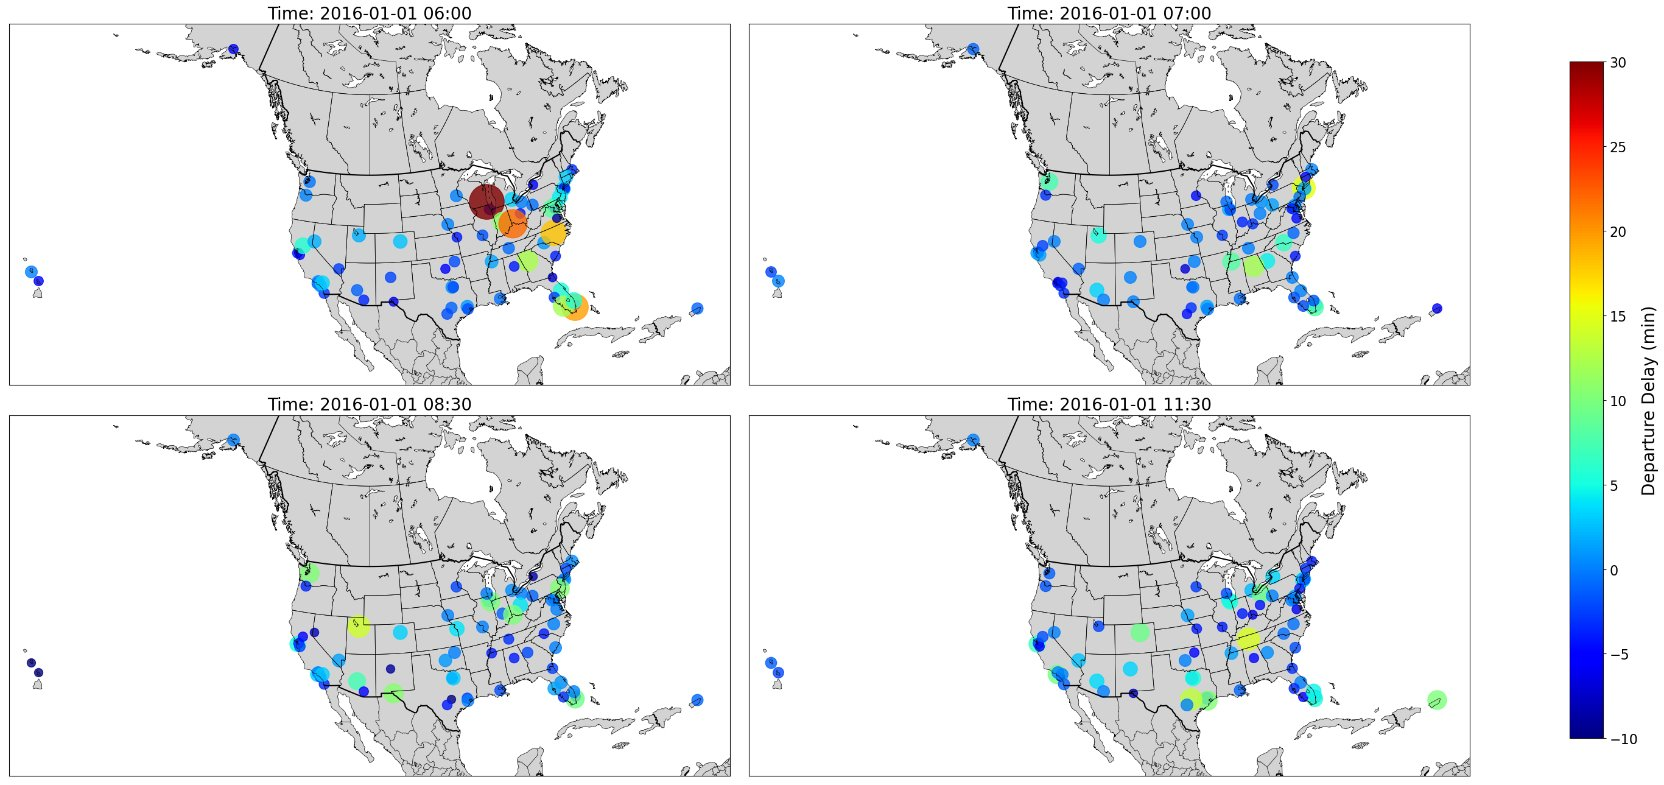
\includegraphics[width=0.85\linewidth]{Spatial-Temporal Airline Delay Data.png}
    \caption{Spatial-Temporal Airline Delay Data of US Airport}
    \label{fig:Spatial-Temporal Data}
\end{figure*}

As illustrated in Fig. \ref{fig:Spatial-Temporal Data}, which depicts a sequence of maps from January 1, 2016, at four different timestamps: 06:00, 07:00, 08:30, and 11:30. This dataset records both arrival and departure delays at various airports. Each map utilizes a color gradient to represent delay duration, where the spectrum extends from deep red, indicating delays exceeding 25 minutes, to deep blue, signifying no delays or instances of early arrivals. This visual representation enables us to meticulously analyze the temporal and geographical variations in airport delays. This furnishes robust data-driven support for our deep learning model, enhancing its predictive accuracy in forecasting flight dynamics.

Moreover, this dataset enables the extraction of specific departure and arrival delay times for designated airports, as demonstrated in Fig. \ref{fig: SFO Delay Data}. From the data we have collected, it is evident that there are certain underlying cyclical patterns in airport delays. We can utilize deep learning models to uncover these patterns by analyzing the data.


\begin{figure}
    \centering
    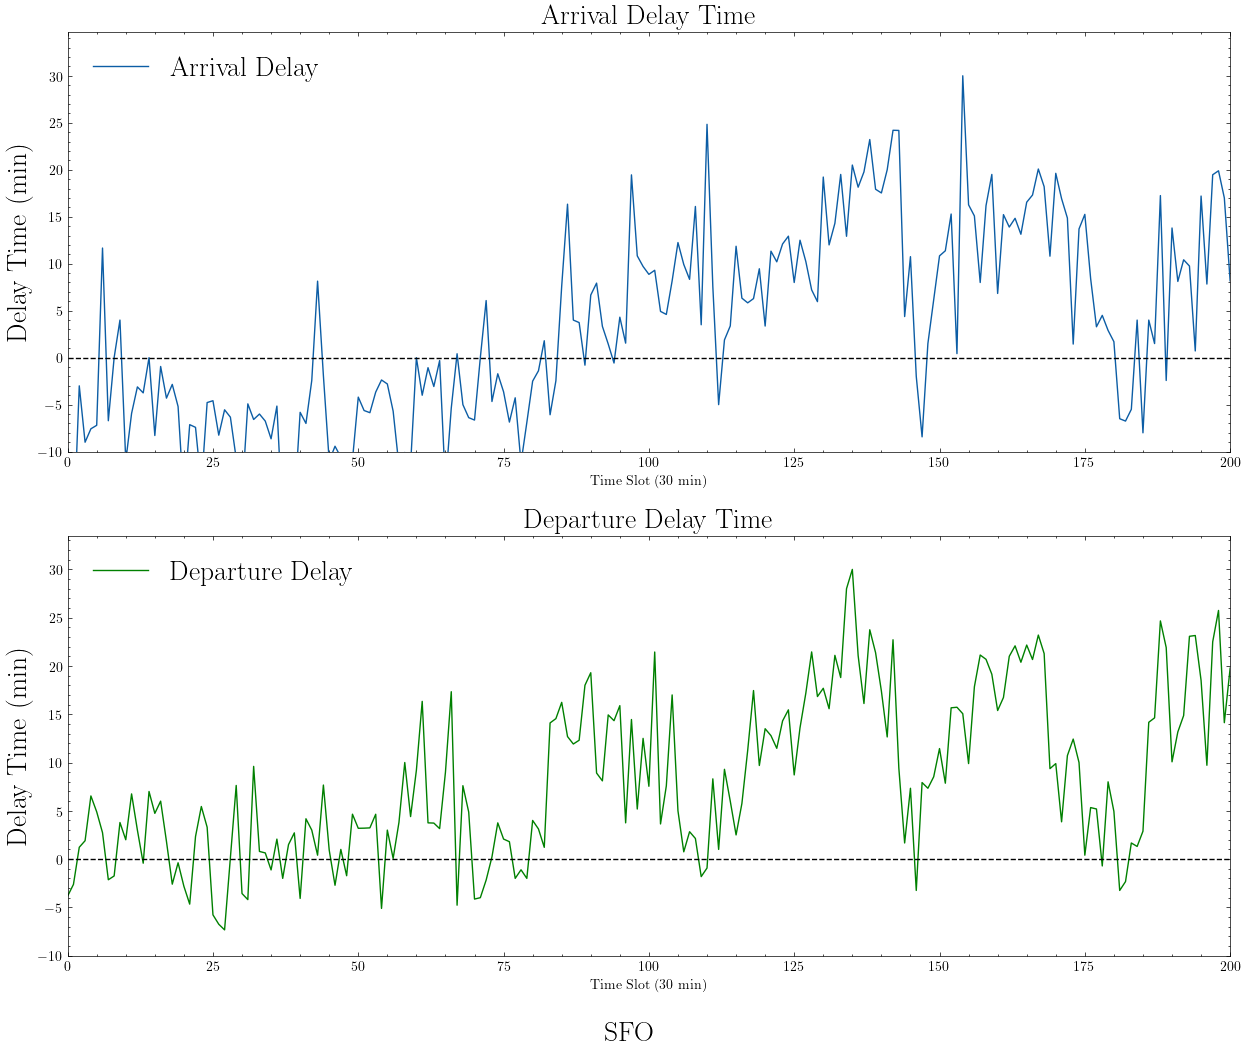
\includegraphics[width=1\linewidth]{SFO.png}
    \caption{Arrival and Departure Delay Data of SFO Airport}
    \label{fig: SFO Delay Data}
\end{figure}

\subsubsection{Data Preprocessing Methodology}

In addressing missing values within our dataset, we adopted a uniform approach by imputing a value of zero for any instances where data was absent. This method ensures consistency in our dataset, facilitating further analysis without introducing bias from the missing data.

Regarding the handling of outlier values in delay times, we implemented a capping strategy. Delay times that exceeded the usual bounds were truncated to fit within a predefined range of -20 to 30 minutes. This range was selected based on the distribution of delay times within our dataset, where values beyond this range were exceedingly rare. Consequently, any delay time exceeding 30 minutes was set to 30 minutes. This approach minimizes the impact of extreme outliers on the overall analysis, thereby maintaining the integrity and reliability of our prediction model.


\section{LLM Implementation}

Insurance-GPT is engineered to analyze potential purchase intent during interactions with users. It is designed to combine specialized task performance with robust general conversational abilities. To achieve this, we have structured the task into three main sub-tasks:
\begin{itemize}
\item \textbf{Basic insurance industry QA capabilities:} This sub-task focuses on understanding and addressing common inquiries within the insurance sector, thereby providing accurate and valuable information to users. We employ the \textit{insuranceQA-v2} dataset to assess the LLM's performance in this area.

\item\textbf{User sentiment analysis:} Recognizing underlying emotions in user dialogues enables us to tailor our responses and recommendations more effectively. For this purpose, we utilize the \textit{Twitter US Airline Sentiment Dataset} as a measure of the LLM’s capability in sentiment analysis.

\item \textbf{Identifying insurance purchase intent:} This involves analyzing user-provided information to determine their likelihood of purchasing travel insurance. We assess the LLM's effectiveness in this area using the 
\textit{Travel Insurance Dataset}.
\end{itemize}

\subsection{Experiment Design}

The experimental framework was supported by the Llama Factory \cite{zheng2024llamafactory}, utilizing its VLLM (Variable Length Language Model) architecture \cite{kwon2023efficient} which enhances the efficiency of the training process and reduces memory usage. The computational demands of the tasks were managed using 4 NVIDIA GeForce RTX 3090 GPUs and Apple M1 Max.

\subsubsection{Fine-tuning on insuranceQA-v2}

Initially, the model underwent supervised fine-tuning (SFT) using the \textit{insuranceQA-v2} dataset to bolster its comprehension of insurance-related queries. This stage was primarily focused on training the LLM to respond accurately to insurance-specific questions, thus improving its domain-specific efficacy.

\subsubsection{Fine-tuning on RLHF data with ORPO}

We implemented the Odds Ratio Preference Optimization (ORPO) \cite{hong2024orpo} technique to streamline the fine-tuning process, thereby enhancing the model's ability to generalize and align with human preferences. ORPO integrates preference alignment directly into the training objective, simplifying the training pipeline and reducing the resources required. This method effectively eliminates the need for separate stages of supervised fine-tuning and reinforcement learning, providing a practical and scalable approach to enhancing LLM performance while ensuring ethical alignment with human values.

\subsubsection{Fine-tuning on Travel Insurance Dataset with LoRA}

In the final step, we fine-tuned the model further on the \textit{Travel Insurance Dataset} using the LoRA technique to increase its precision in predicting user intent to purchase travel insurance. This step builds on the previous adjustments, aiming to refine the model's predictive accuracy.


\subsection{Retrieval-Augmented Generation: Using ChatOllama to Implement Localization RAG}

ChatOllama \footnote{\url{https://python.langchain.com/v0.1/docs/integrations/chat/ollama/}} is an open-sourcing project based on the Ollama \footnote{\url{https://github.com/ollama/ollama}}, which can help us to localize the LLM, chat with models conveniently and create a knowledge base quickly.

\subsubsection{Setup the Ollama and import the model}
We first git clone the ollama from github to fetch the llama.cpp, which can help us to import a model from Pytorch and safetensors. After we install the Python dependencies, we can build the quantize tool. And we will use the convert.py in the \verb|llama.cpp| to convert the model to GGUF, then we quantize the convert result so that we can deploy the model in most devices to chat, though we think this process will decrease our LLM's performance. 

\subsubsection{Create the model and test with the prompt}
After importing the fine-tuning model into a \verb|quantized.bin|, we will use the Ollama method to create a model with the prompt we designed,
\begin{Verbatim}[breaklines=true]
FROM InsuranceGPT
# set the temperature to 1 [higher is more creative, lower is more coherent]
PARAMETER temperature 0.5
# set the system message
SYSTEM """
Assistant is an expert agent about the flight info designed to assist with a wide range of tasks, including providing the predicted delay and flight insurance recommendations.
Assistant should ask for the user information about the flight departure or arrival, the user name only at the beginning of the conversation with users.
....
\end{Verbatim}
 we can test it in the ChatOllma interface.

\subsubsection{Create the knowledge base and run together}
The ChatOllma has a quick knowledge base creating method, we just need to supply the file(PDF, word, etc.) and choose the embedding model, we choose the nomic-embedding model here since the nomic-embedding model beat the OpenAI's Ada-002 and text-embedding-3-small in the long sequence text. The nomic-embedding model is based on the BERT but replaced absolute position embedding with rotational position embedding to support long sequences and use SwiGLU activation instead of GeLU for faster training. We can create the knowledge base within 1 minute for about 10 pages of PDF. Finally, we can choose the knowledge base we need with our model to chat.

\section{Deep Learning Model}

The objective is to design a time series prediction deep learning model and encapsulate the entire model into a module, where the LLM can be conveniently invoked after obtaining the corresponding query. 

Given the unique nature of airport network data, which includes complex temporal and spatial relationships, traditional time series prediction models struggle to handle it effectively. Therefore, we attempt to use graph learning models to improve prediction accuracy. In the field of spatio-temporal graph prediction, there is already a considerable amount of research. ASTGCN \cite{guo2019attention} is a relatively classic early architecture. It combines attention mechanisms with graph convolution to extract spatio-temporal correlations, thereby improving prediction accuracy. The original ASTGCN framework was designed to predict road traffic flow. In our project, we adapted this framework to suit our dataset through some modifications.

As illustrated in Fig. \ref{fig:ASTGCN}, the ASTGCN framework is specifically engineered to manage large datasets through the integration of two spatial-temporal blocks. This structure is enhanced with residual connections to preserve the integrity of input data, which is crucial for building deeper neural networks.

% \begin{figure}[h!]
%     \centering
%     \begin{subfigure}[b]{0.45\linewidth}
%         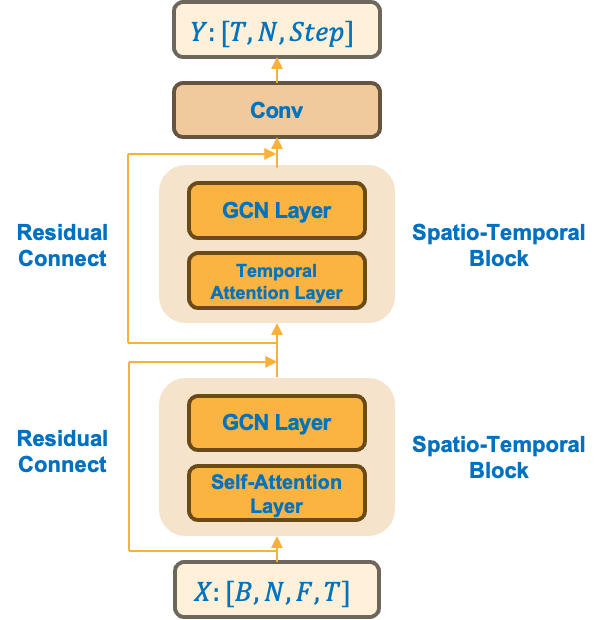
\includegraphics[width=\linewidth]{ASTGCN.png}
%         \caption{Framework of ASTGCN}
%         \label{fig:ASTGCN}
%     \end{subfigure}
%     \hfill
%     \begin{subfigure}[b]{0.5\linewidth}
%         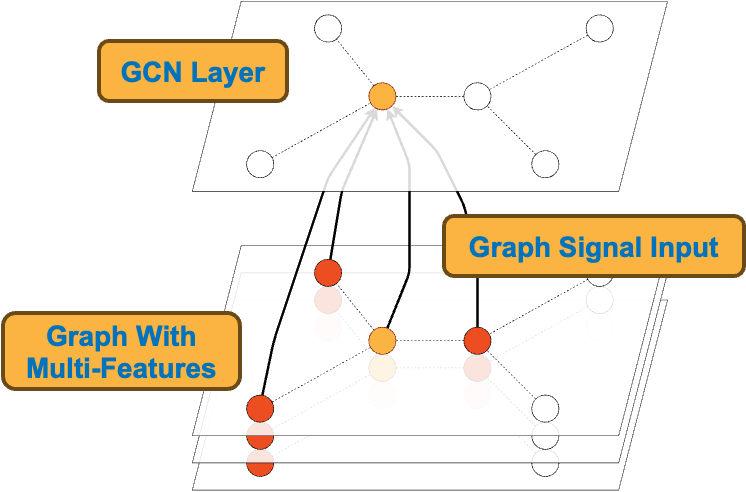
\includegraphics[width=\linewidth]{gcn.png}
%         \caption{Graph Convolutional Network}
%         \label{fig:gcn}
%     \end{subfigure}
%     \caption{Structure}
%     \label{fig:overall-label}
% \end{figure}

\begin{figure}[h]
    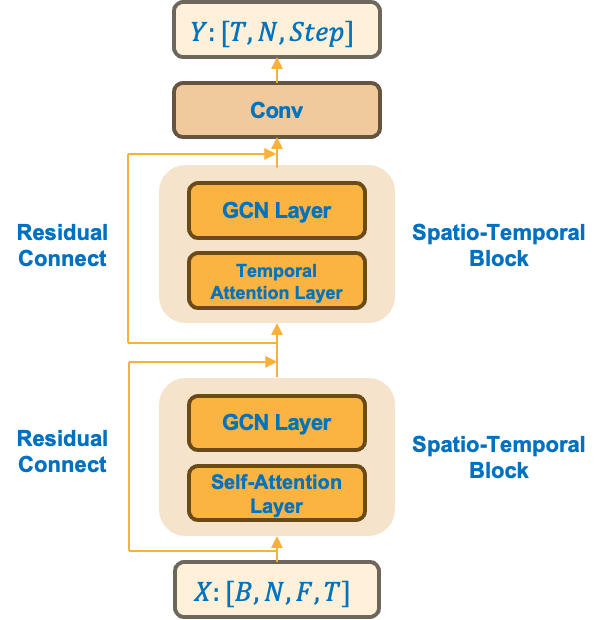
\includegraphics[width=0.8\linewidth]{ASTGCN.png}
    \caption{Framework of ASTGCN}
    \label{fig:ASTGCN}
\end{figure}



\subsection{Spatio-Temporal Block}

The core component of the ASTGCN model is the Spatial-Temporal Block, which employs a self-attention layer to effectively capture both spatial and temporal correlations within the data. This dual-focus mechanism is critical for addressing different aspects of the data's dynamics:
\begin{itemize}

\item \textbf{Temporal Correlation:} Within the temporal dimension, the model identifies and leverages correlations across different time slices. This is particularly vital in applications such as flight data analysis, where conditions evolve significantly over time.

\item \textbf{Spatial Correlation:} Spatially, the influence of individual nodes (e.g., airports) varies, with certain nodes exerting a more significant impact on the overall system due to factors such as weather conditions or passenger flow. Understanding these disparities is essential for accurate predictions and analyses.
\end{itemize}
\subsection{Graph Convolutional Network}


Following the application of the self-attention layer, the model constructs a comprehensive graph that encapsulates multi-spatial and temporal features, integrating these complex relationships into a unified data representation. This enriched graph is then processed through a Graph Convolutional Network (GCN), which operates similarly to traditional Convolutional Neural Networks (CNNs) but is specifically designed to handle graph-structured data. As illustrated in Fig. \ref{fig:gcn}, the GCN layer aggregates information not only from each node but also from its adjacent nodes, effectively capturing both local interactions and global structural dynamics within the graph.

The integration of the GCN within the ASTGCN framework allows for sophisticated processing that simultaneously convolves across spatial and temporal dimensions. This capability is crucial for interpreting the complex interdependencies and evolving patterns inherent in the data, enabling the ASTGCN model to pinpoint specific attributes of individual nodes while also understanding the broader interconnections that define the entire network's functionality. As a result, the ASTGCN model emerges as a robust tool for complex data analysis tasks, providing a nuanced understanding of both temporal trends and spatial hierarchies essential for accurate decision-making and prediction in dynamic systems.

\begin{figure}[h]
    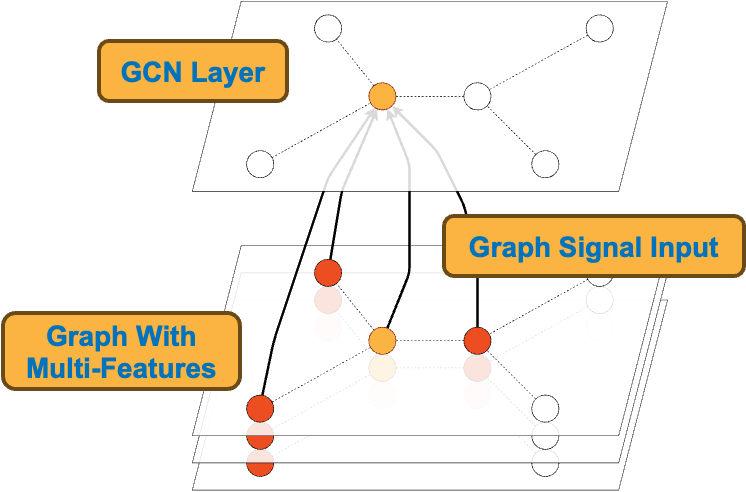
\includegraphics[width=0.8\linewidth]{gcn.png}
    \caption{Graph Convolutional Network}
    \label{fig:gcn}
\end{figure}


\section{Result Analysis}

\subsection{Main Result}

\subsubsection{LLM Part}



\begin{table*}[h!]
\caption{The Main Result of Insurance-GPT}

\label{baseline}
\fontsize{8pt}{13pt}\selectfont % This line changes the font size and line spacing
\begin{tabular}{cccccccccc}
\toprule
                                              & \multicolumn{2}{c}{Travel Insurance}                                        & \multicolumn{2}{c}{Travel Insurance (with 4 labels)}                         & \multicolumn{2}{c}{Twitter US Airline Review}                               & \multicolumn{3}{c}{insuranceQA-v2}                                                                                   \\ \cline{2-10} 
\multirow{-2}{*}{Model}                       & Accuracy                             & F1 Score                             & Accuracy                             & F1 Score                             & Accuracy                             & F1 Score                             & ROUGE-1                               & ROUGE-2                              & ROUGE-N                               \\ \hline
GPT-3.5                                       & 0.58                                 & 0.23                                 & 0.4                                  & 0.18                                 & 0.73                                 & 0.42                                 &                                       &                                      &                                       \\
Llama3                                        & 0.61                                 & 0.2                                  & 0.09                                 & 0.07                                 & 0.67                                 & 0.53                                 & {\color[HTML]{CB0000} \textbf{28.21}} & 5.69                                 & 15.24                                 \\
{\color[HTML]{000000} \textbf{Insurance-GPT}} & {\color[HTML]{CB0000} \textbf{0.75}} & {\color[HTML]{CB0000} \textbf{0.71}} & {\color[HTML]{CB0000} \textbf{0.63}} & {\color[HTML]{CB0000} \textbf{0.37}} & {\color[HTML]{CB0000} \textbf{0.81}} & {\color[HTML]{CB0000} \textbf{0.73}} & 25.49                                 & {\color[HTML]{CB0000} \textbf{6.50}} & {\color[HTML]{CB0000} \textbf{16.21}} \\ \toprule
\end{tabular}

\end{table*}

During the evaluation phase, as detailed in TABLE \ref{baseline}, we conducted a comparative analysis of Insurance-GPT against the Llama3 and GPT-3.5 models. The comparative results consistently demonstrated that Insurance-GPT achieved the highest accuracy across tasks, including predicting insurance purchase intent and analyzing review sentiments. Notably, Insurance-GPT's exceptional F1 scores, indicative of its precision and recall, underscore its capability to precisely identify relevant instances while effectively minimizing false positives and negatives.

Interestingly, despite the absence of specific fine-tuning on datasets such as the Twitter US Airline Sentiment and Travel Insurance (with 4 labels), Insurance-GPT markedly outperformed the baseline models. This performance accentuates the inherent generalization capabilities of large language models, trained on broad and varied datasets, to adeptly manage zero-shot tasks that were not explicitly covered in their training regime \cite{wei2022finetuned}. These outcomes affirm the robustness and adaptability of LLMs, showcasing their capacity to transfer learned knowledge to novel and unencountered challenges without the necessity for explicit task-specific training.

The similar ROUGE scores between Insurance-GPT and Llama3 on the insuranceQA-v2 dataset suggest that specialized fine-tuning may sometimes compromise a model's general conversational abilities. This observation raises the possibility of a trade-off between domain-specific accuracy and broader linguistic flexibility, which we intend to further explore in our forthcoming ablation study. This study aims to identify optimal training strategies that balance specialized performance with general applicability.

\begin{figure}[h]
    \centering
    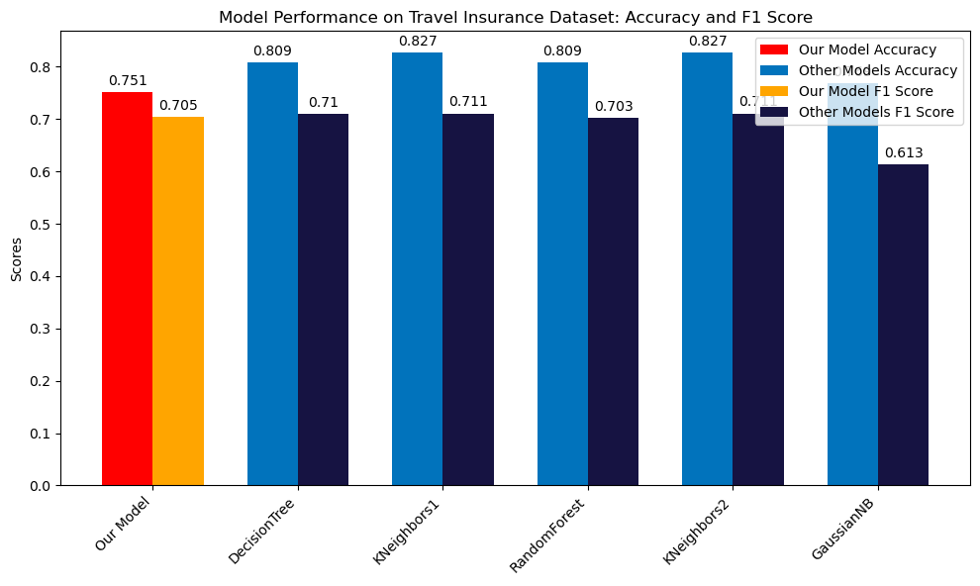
\includegraphics[width=1\linewidth]{baseline model.png}
    \caption{Comparative Analysis of Numerical Models}
    \label{fig:baseline}
\end{figure}

Furthermore, we extended our comparative framework to include various numerical models: Decision Tree, K-Neighbors, Random Forest, Logistic Regression, and Gaussian-NB. The outcomes, as depicted in Fig. \ref{fig:baseline}, revealed that the F1 scores of these traditional numerical prediction models were comparable to those of Insurance-GPT. This underscores the robust capabilities of Insurance-GPT, demonstrating that it excels not only in linguistic tasks but also exhibits strong potential in numerical predictive modeling, showcasing its versatility and efficacy across different types of data analytics tasks.


\subsubsection{Deep Learning Model Part}

% ASTGCN todo
\begin{figure}[h]
    \centering
    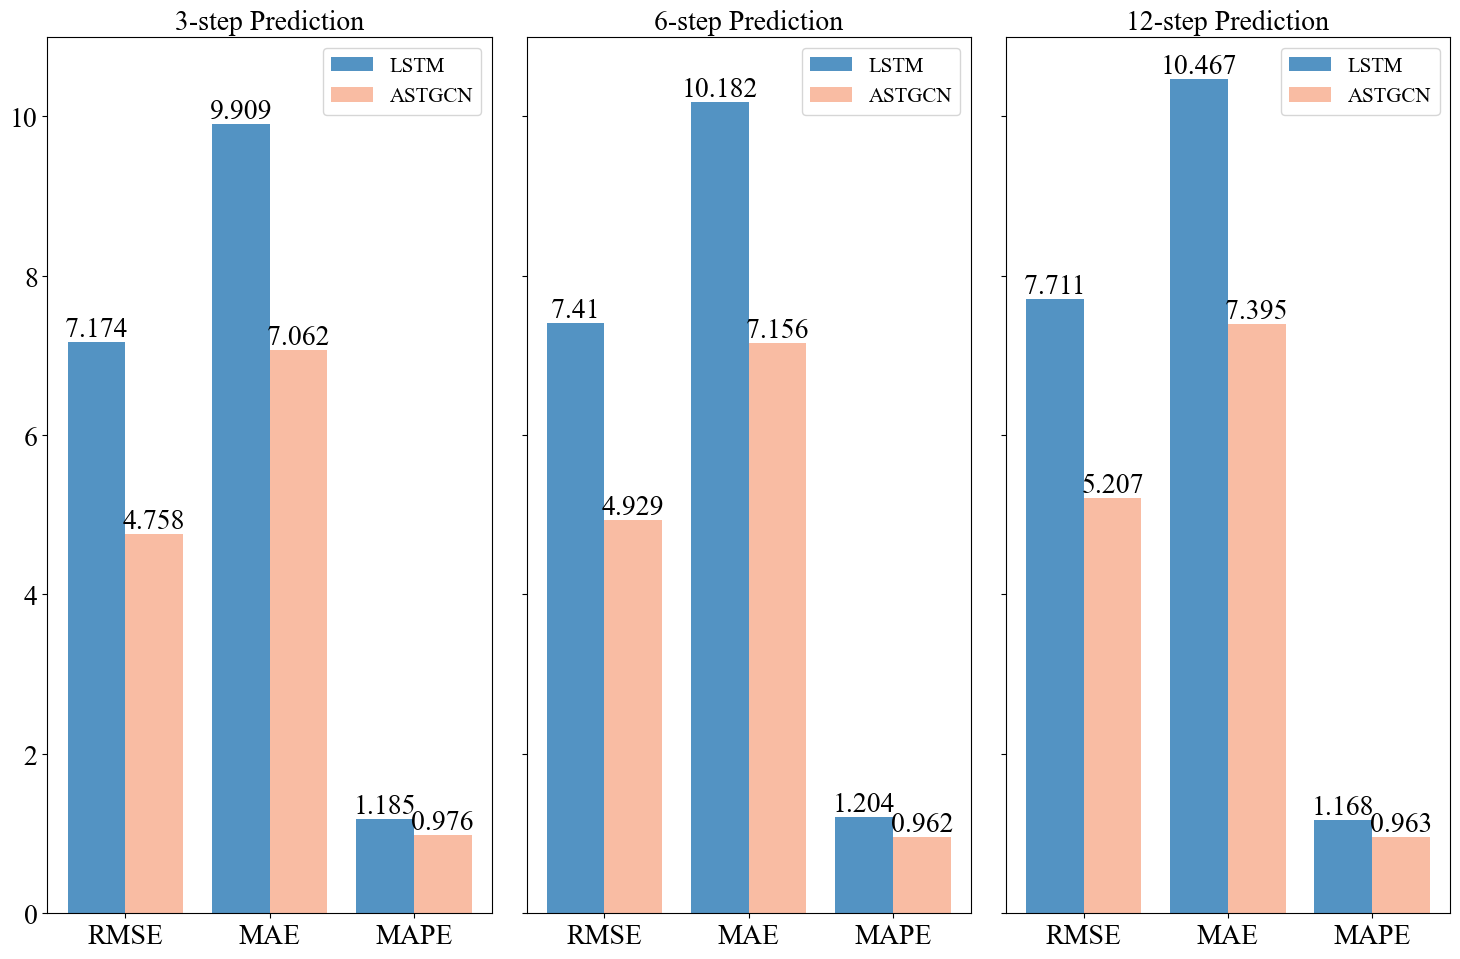
\includegraphics[width=1\linewidth]{eval.png}
    \caption{Metrics Results}
    \label{fig:Metrics}
\end{figure}

To benchmark the performance of our model, we compared it with a traditional LSTM model using three key metrics: Root Mean Square Error (RMSE), Mean Absolute Error (MAE), and Mean Absolute Percentage Error (MAPE). These metrics were chosen due to their ability to provide a comprehensive quantification of prediction accuracy and error magnitude in forecasting tasks.

Fig. \ref{fig:Metrics} below illustrates the evaluation results. It is evident from the metrics that our model consistently outperforms the LSTM baseline, achieving lower scores in RMSE, MAE, and MAPE, thereby indicating superior prediction precision and reliability.



% \begin{figure*}[h]
%     \centering
%     \begin{subfigure}{0.5\textwidth}
%         \centering
%         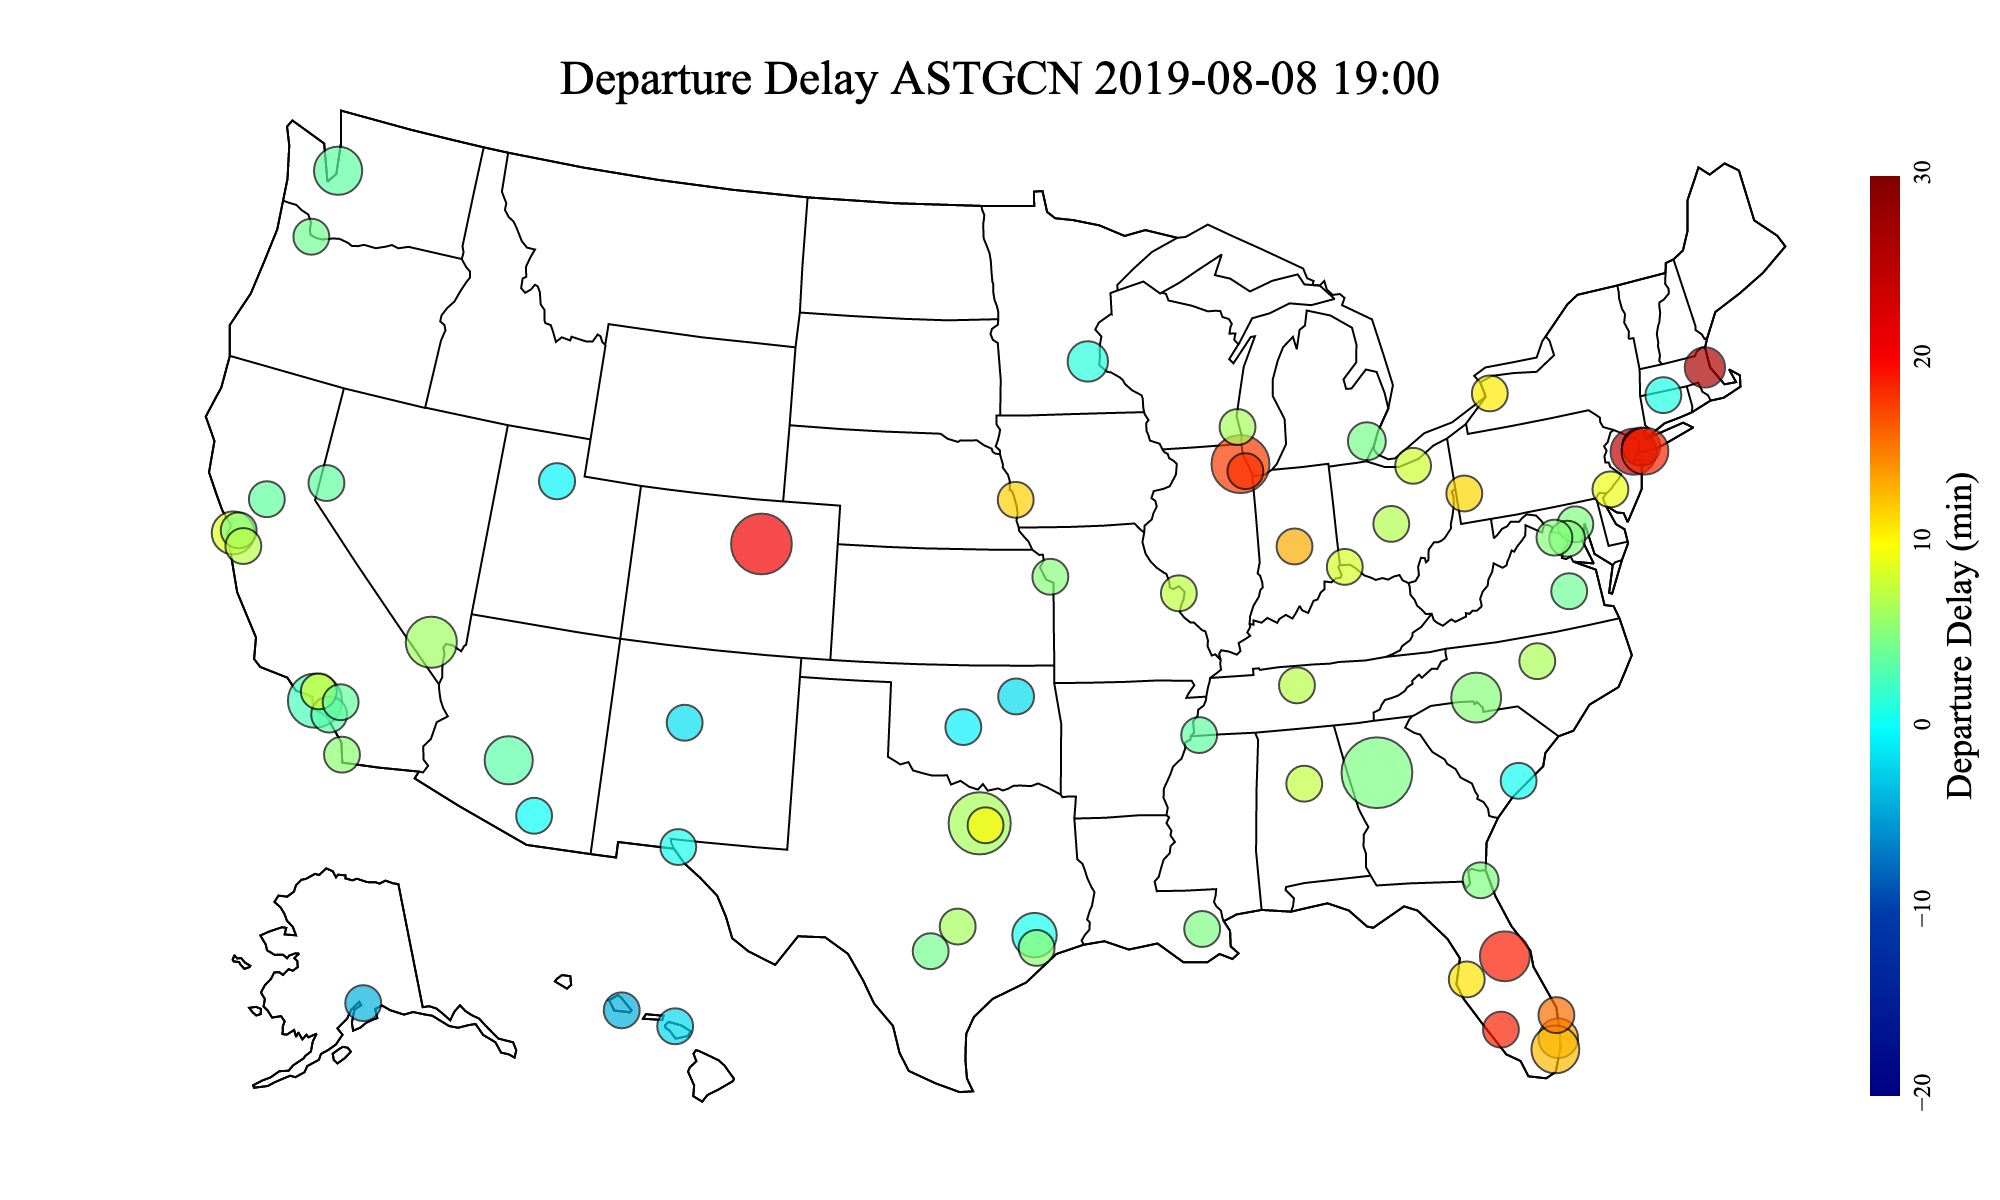
\includegraphics[width=\linewidth]{us_ASTGCN_7.png}
%         \caption{Prediction}
%         \label{fig:sub1}
%     \end{subfigure}%
%     \begin{subfigure}{0.5\textwidth}
%         \centering
%         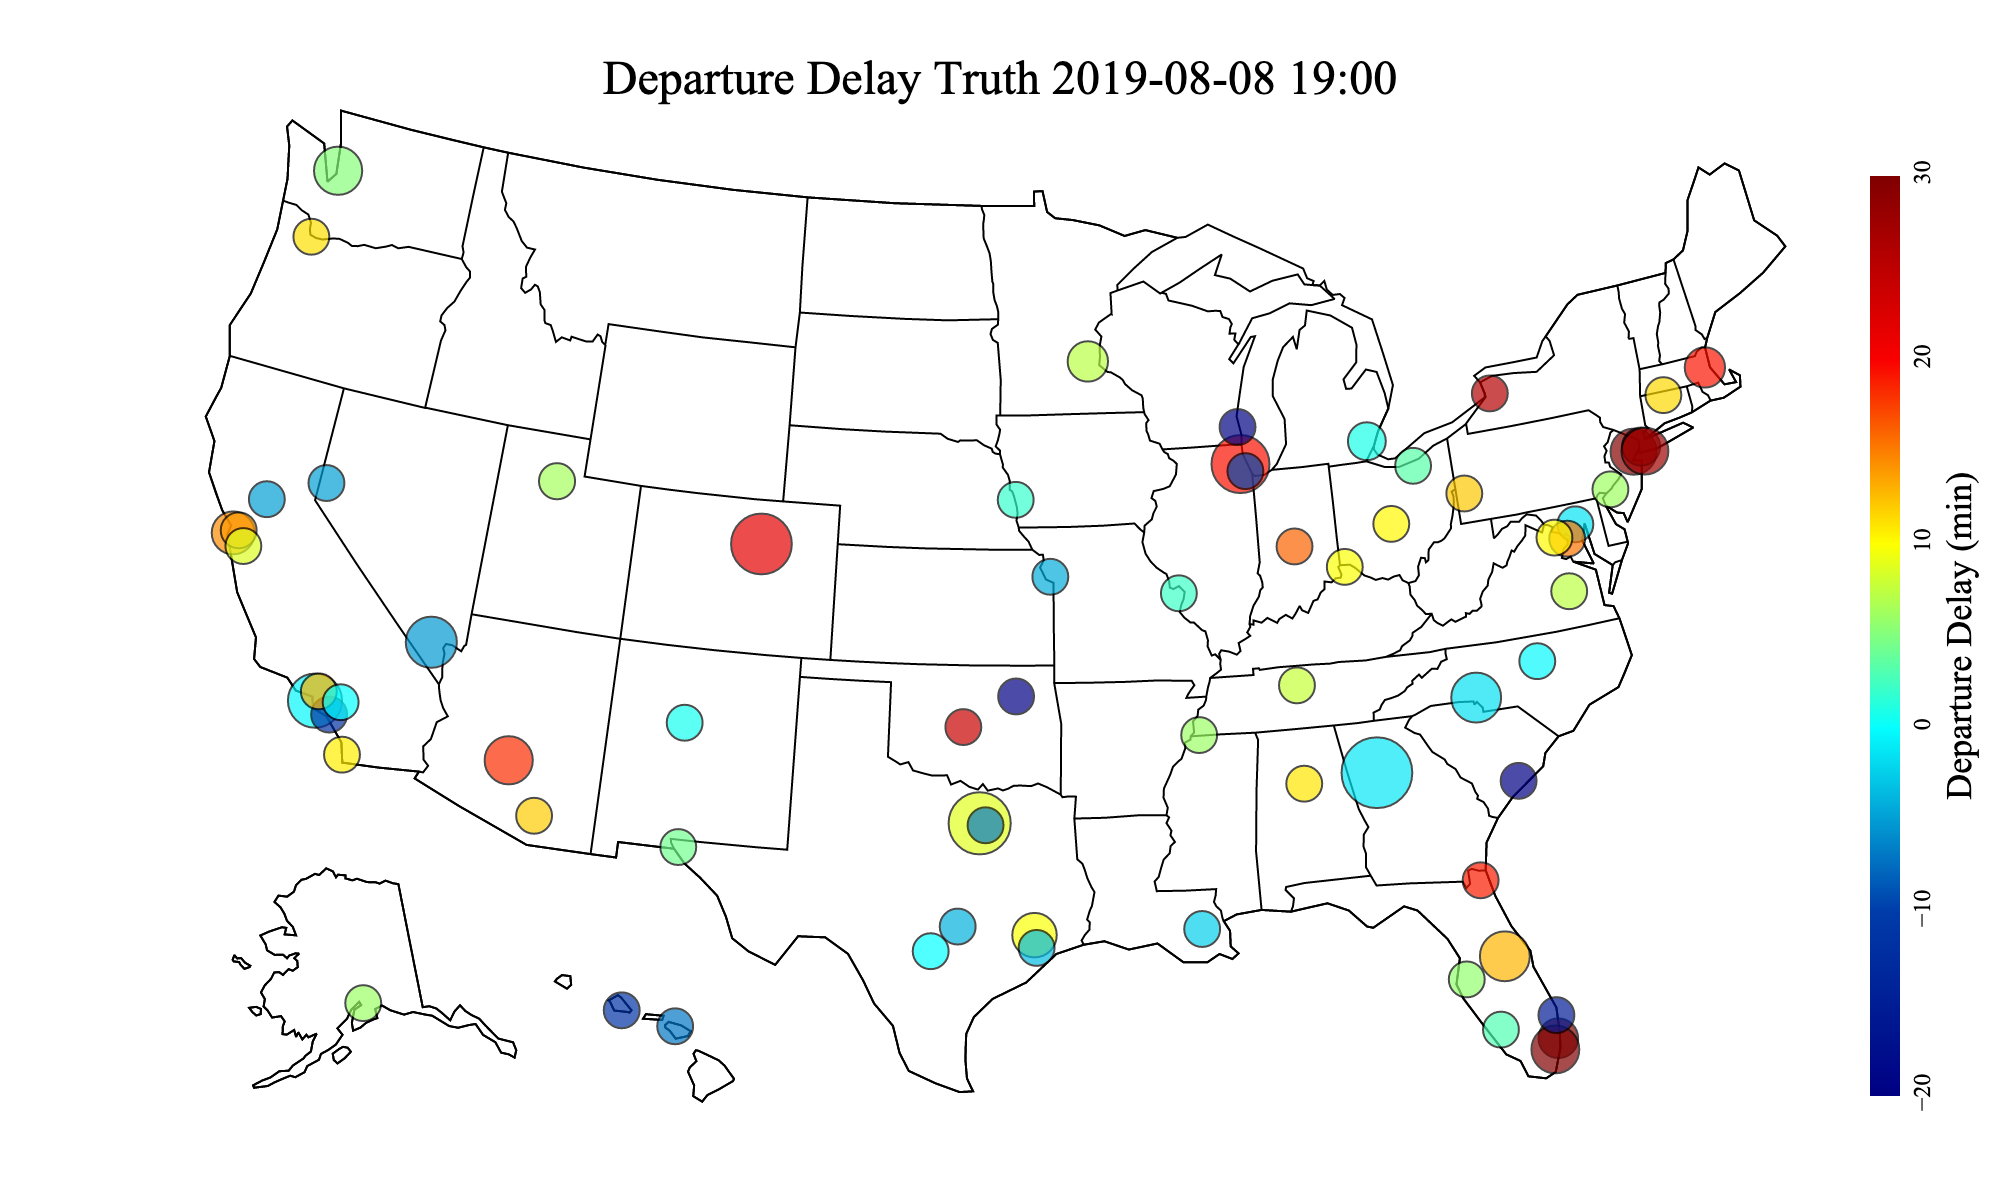
\includegraphics[width=\linewidth]{us_Truth_7.png}
%         \caption{Truth}
%         \label{fig:sub2}
%     \end{subfigure}
%     \caption{Spatial Visualization of Departure Delay}
%     \label{fig:test}
% \end{figure*}

\begin{figure}[h]
    \centering
    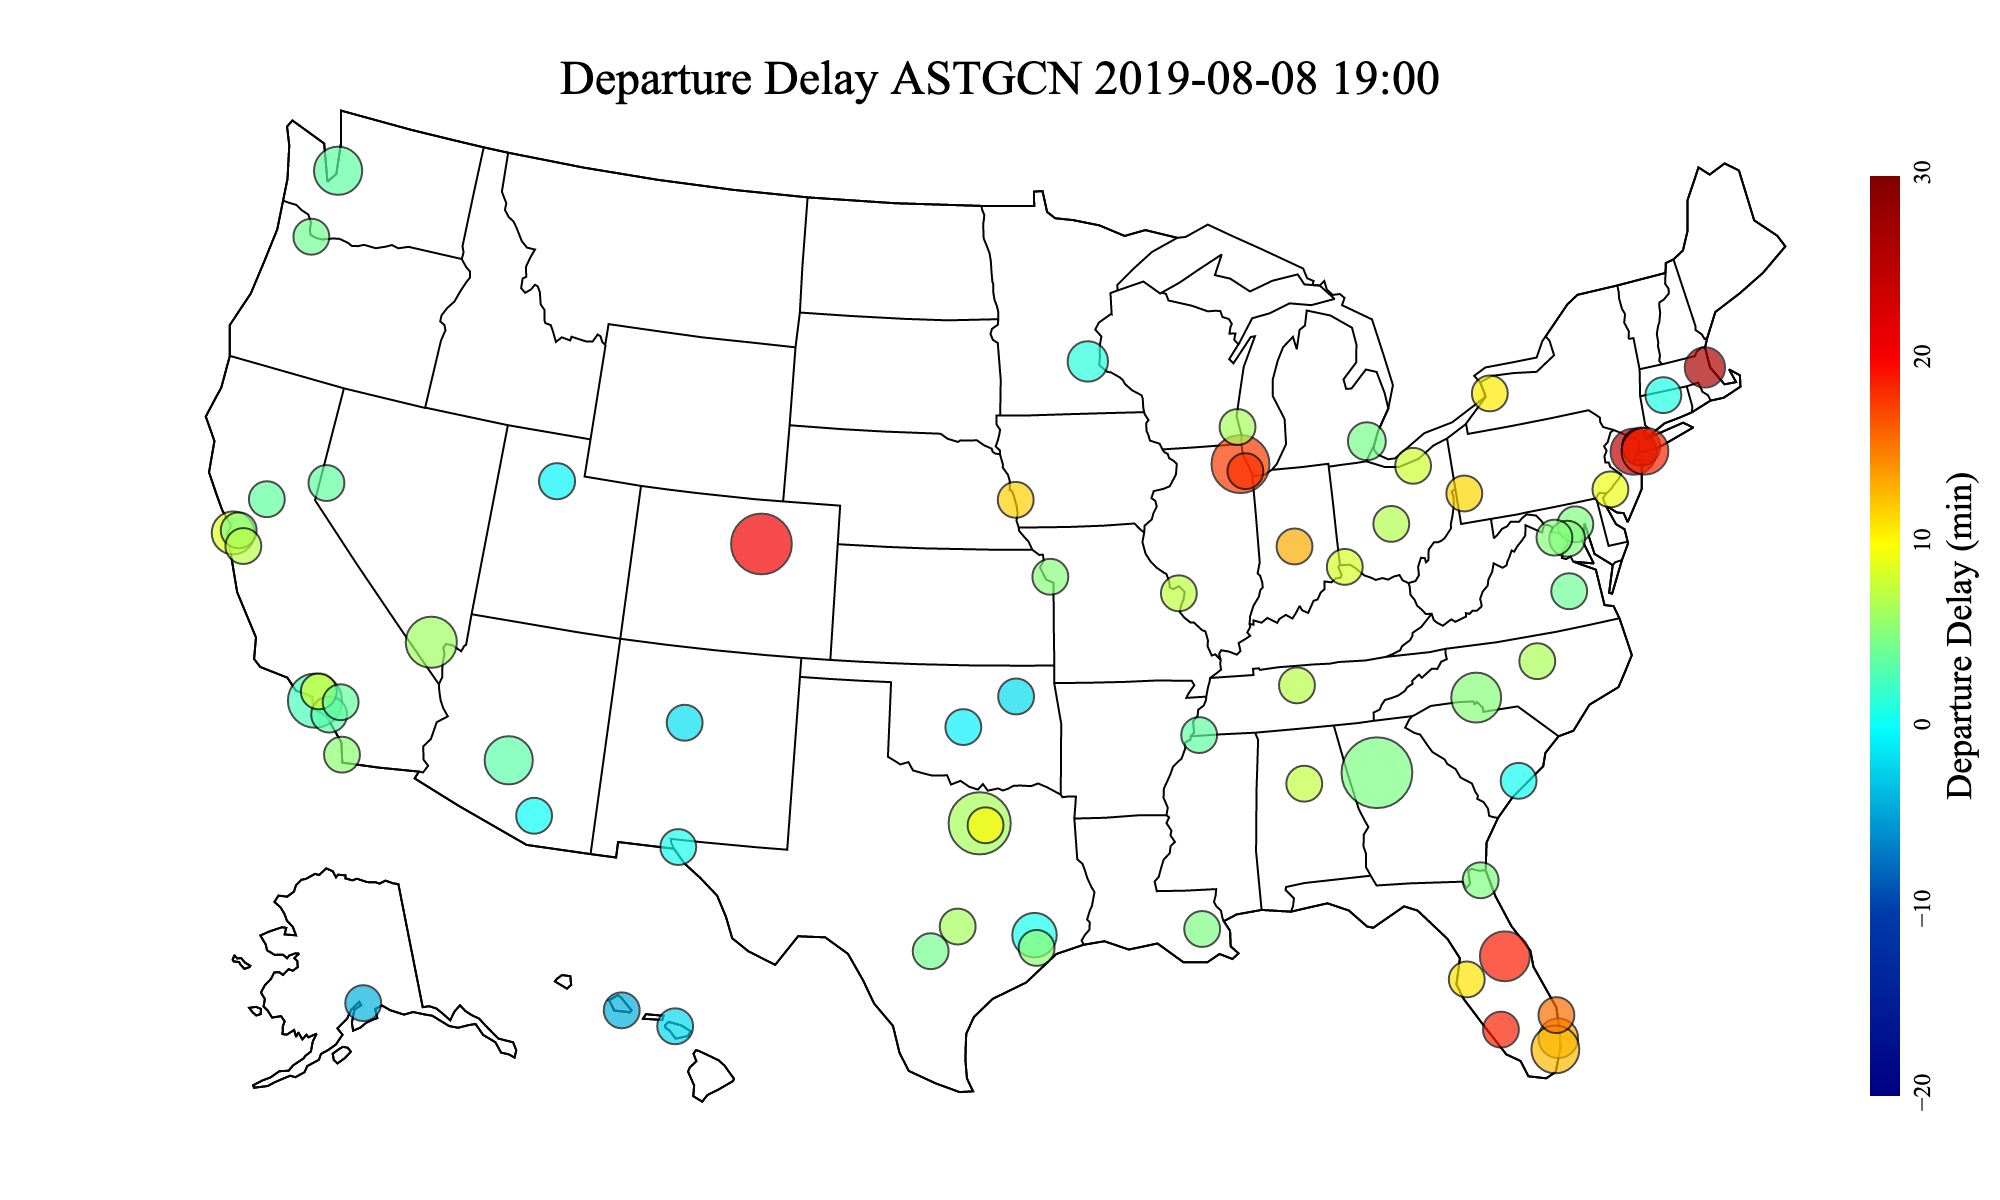
\includegraphics[width=1\linewidth]{us_ASTGCN_7.png}
    \caption{Prediction}
    \label{fig:Prediction}
\end{figure}

\begin{figure}[h]
    \centering
    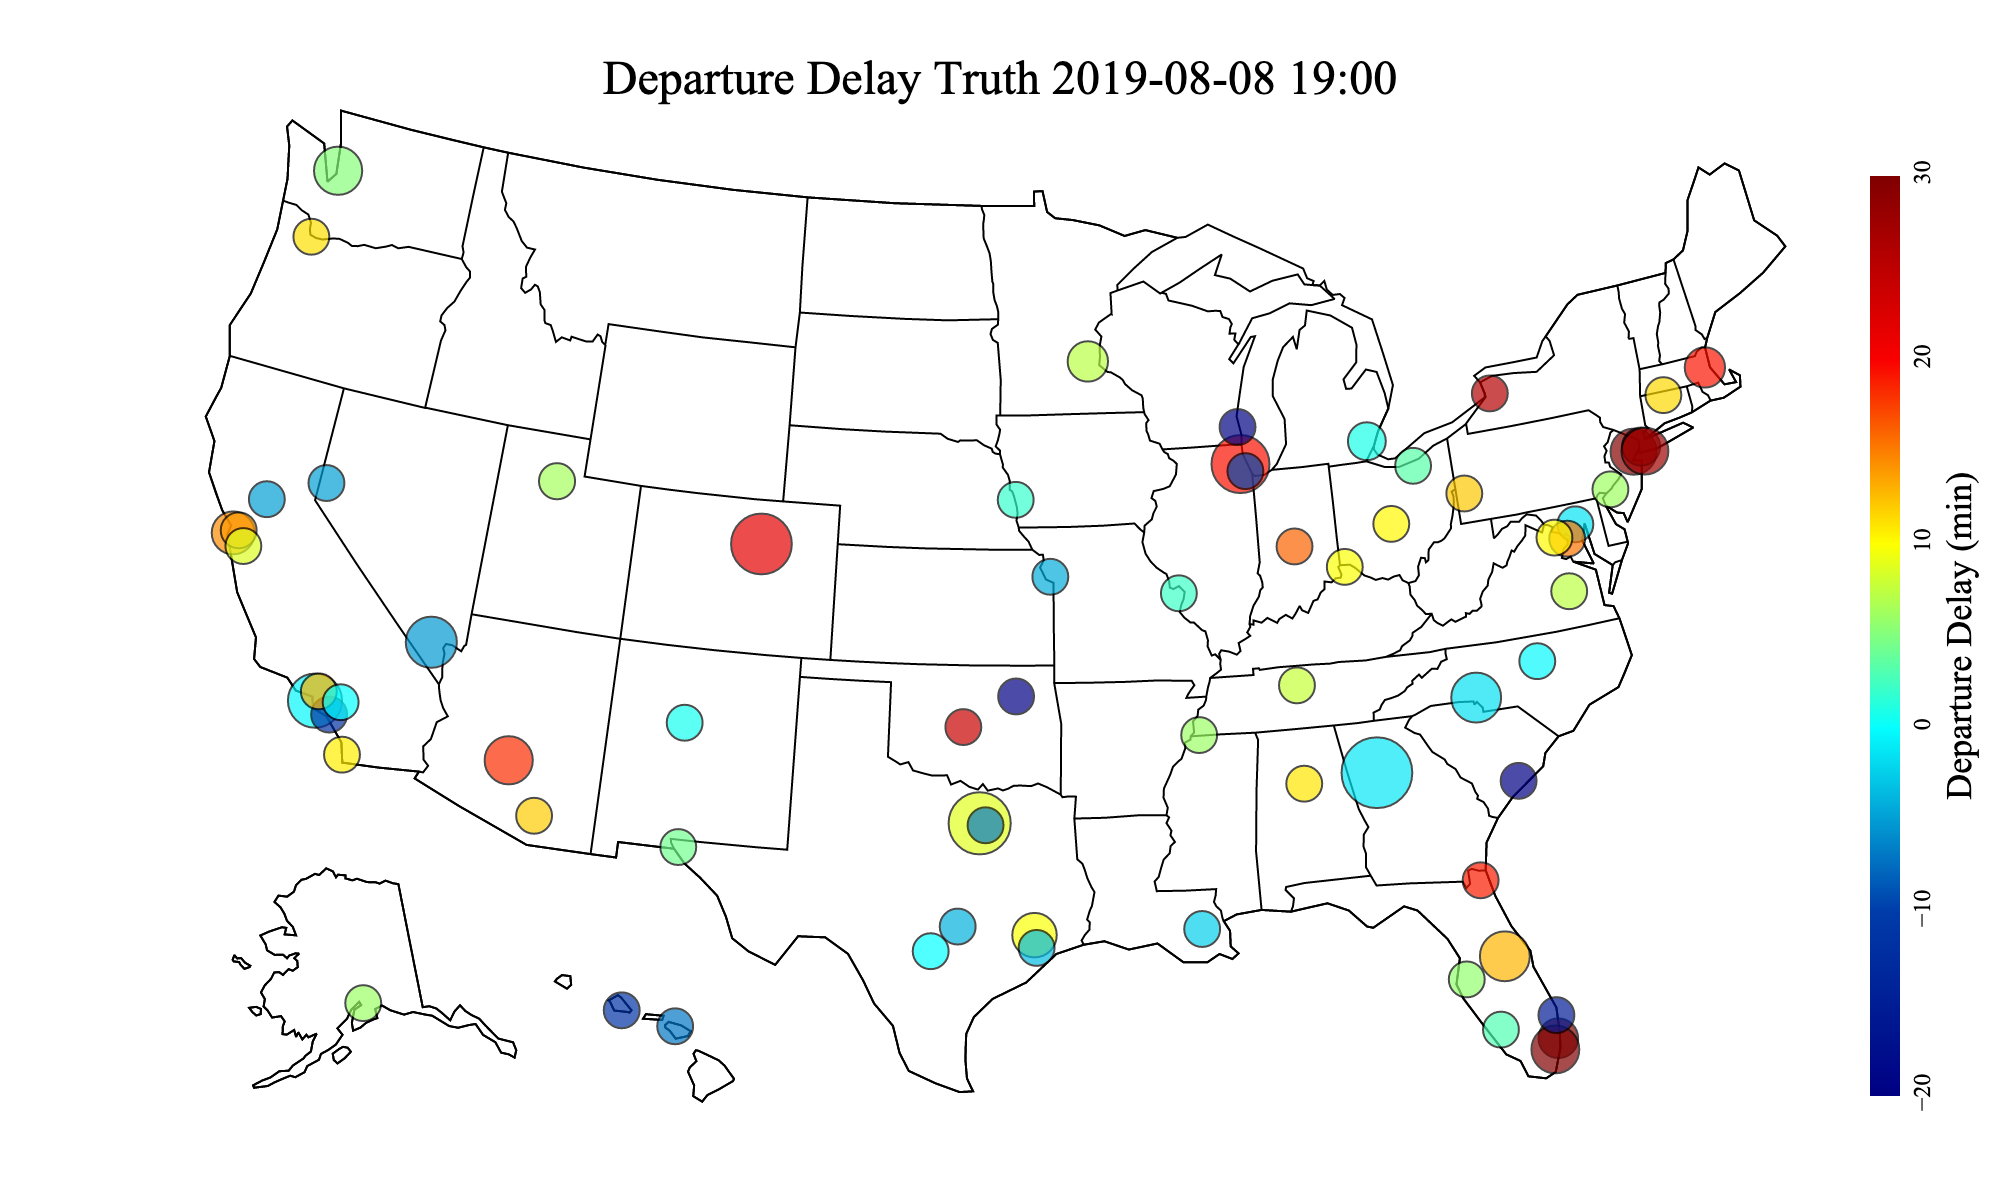
\includegraphics[width=1\linewidth]{us_Truth_7.png}
    \caption{Truth}
    \label{fig:Truth}
\end{figure}

Fig. \ref{fig:Prediction} and Fig. \ref{fig:Truth} provide a spatial visualization of our model’s predictive performance. While the model does not perfectly predict the delay time for every airport node, it accurately forecasts the regional trends in delays. For instance, the delay patterns at airports in the Central and Eastern United States closely match those of the actual data, demonstrating the model's effectiveness in capturing spatial dependencies and regional dynamics.


\begin{figure*}[h!]
    \centering
    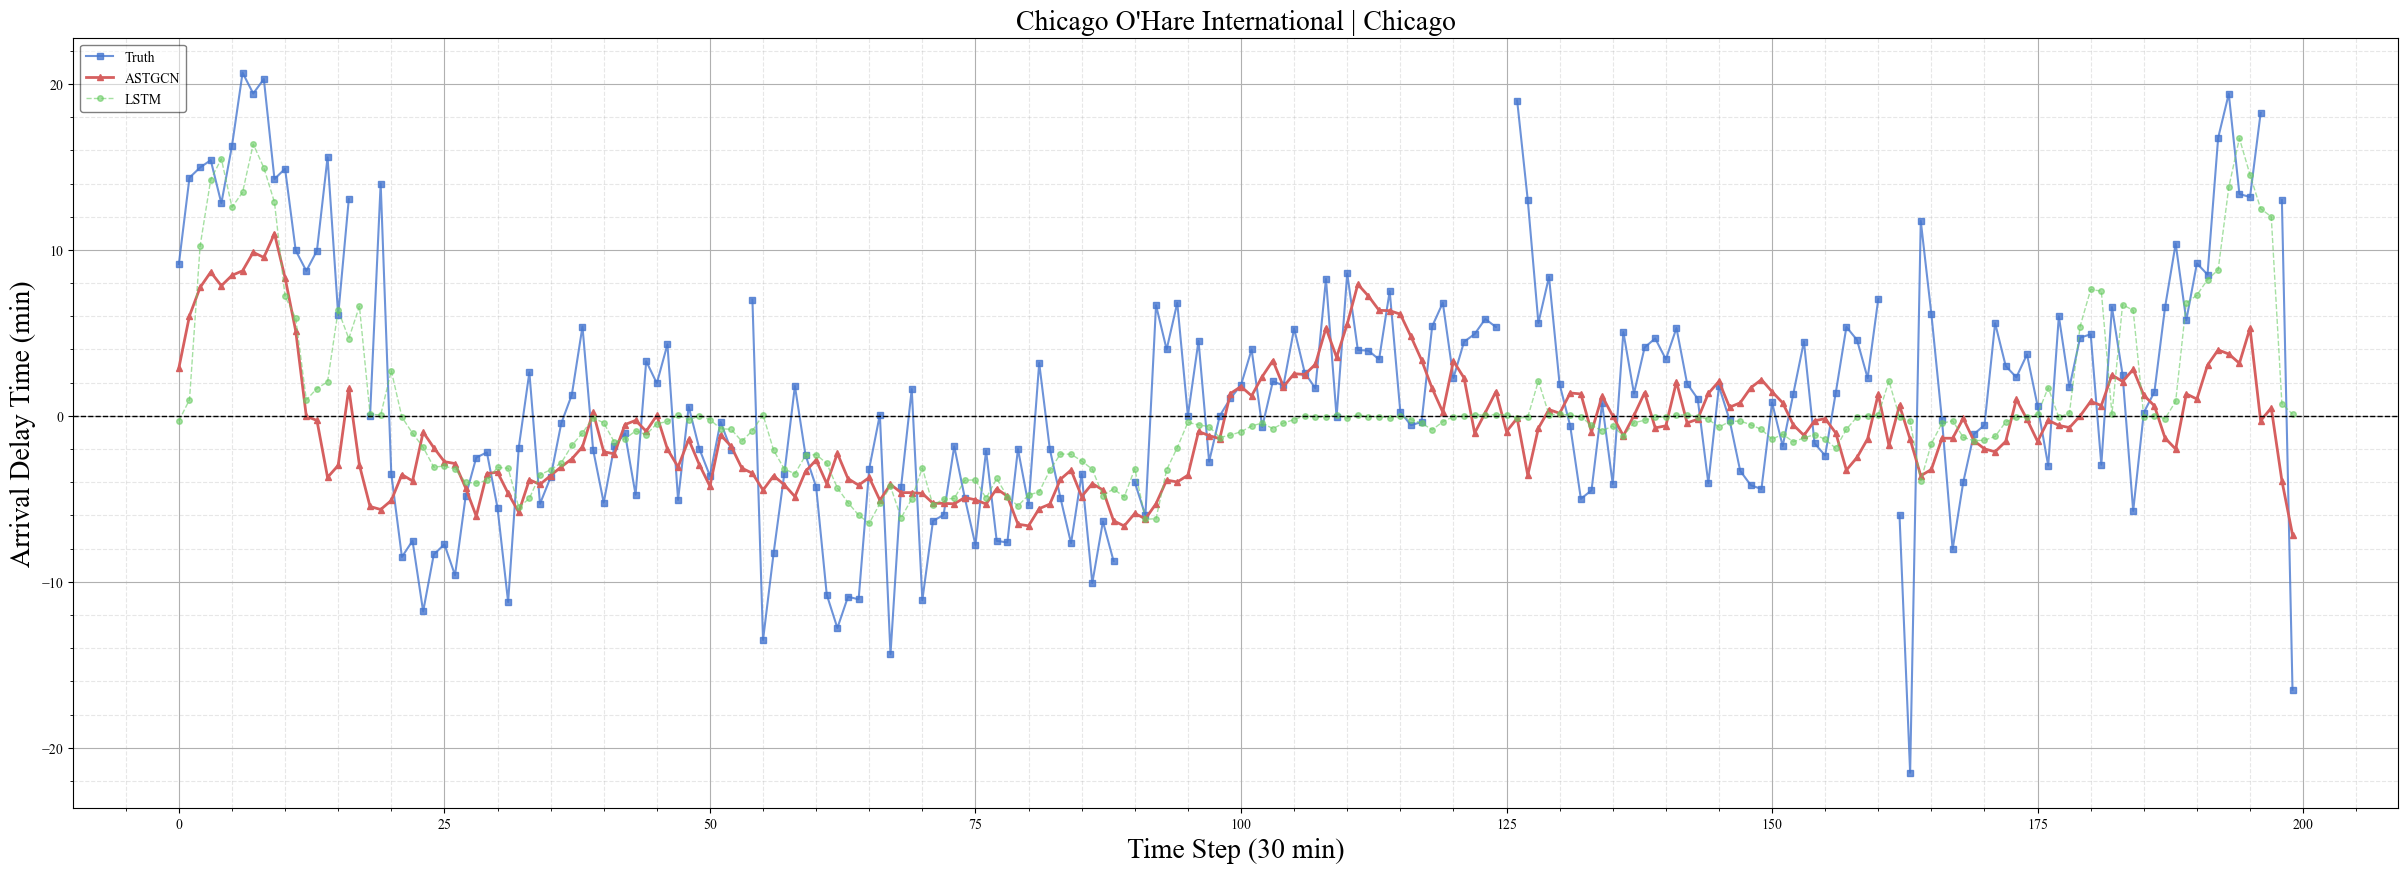
\includegraphics[width=1\linewidth]{temporal.png}
    \caption{Temporal Visualization of Arrival Delay}
    \label{fig:chi}
\end{figure*}

In Fig. \ref{fig:chi}, we present a comparison of the predictive performance of our model versus an LSTM model at Chicago O'Hare International Airport. As illustrated, although the LSTM model can effectively capture fluctuations in airport delays, it falls short in accurately predicting periods with high volatility and less apparent temporal regularities. This demonstrates that our model, by capturing both spatial and temporal correlations, can more effectively analyze the network of airport delays.

This enhanced capability enables our model to provide more reliable forecasts, particularly in complex scenarios where understanding the interplay between different airports and times is crucial. By integrating spatial-temporal dynamics into our analysis, we offer a more robust framework for anticipating and managing variability in airport operations, leading to more informed decision-making in transportation management.


\subsection{Demo}

In Fig. \ref{fig:demo}, we tested an example in ChatOllama. 

\begin{figure}[h!]
\begin{AIbox1}{An example chat history for AI system}
{\bf User:} \\
{\small Hello.}
\tcbline
{\bf Insurance-GPT:} \\
{\small
\textbf{Flight Assistant}\\
Hello! This is the flight assistant. I'm here to help you with your flight-related queries.\\
\textbf{User Information}\\
Unfortunately, we don't have any specific information about your flight yet. Could you please provide me with your name and more details about the flight you're taking?\\
Once I have that information, I'll be happy to assist you with any questions or concerns you may have!
}
\tcbline
{\bf User:} \\
{\small I'm Leggis, and I will take the flight from LAX to BOS, could you tell me will it delay?}
\tcbline
{\bf Flight Assistant:} \\
{\small 
Based on our knowledge base, your flight from \textbf{LAX} to \textbf{BOS} is predicted to have a departure delay of approximately \textbf{79 minutes}.\\
As for the arrival delay, we predict that your flight will arrive at BOS with a delay of around \textbf{85.4 minutes}.\\
Considering your purchase intention level (which is 3). I recommend \textbf{Level 2 insurance} for you. This recommendation is based on our analysis of the predicted delays and your purchase intention.\\
Please let me know if you have any further questions or concerns!
}
\end{AIbox1} 
\caption{The Demo Chat with Insurance-GPT in ChatOllama}
\label{fig:demo}
\end{figure}

You can see when a user wants to query something, the model will act as a role of flight assistant and ask for more user information to supply more help. When the user provides the name, the departure airport, the arrival airport, and the time the flight will departure, the LLM will use a function to get the predicted delay time for departure or arrival:

\begin{lstlisting}[language=Python]
def get_delay_time(airport, time):
    info = get_airport_info(airport)
    airport_idx = info['idx']
    step = 0
    length = 200
    ASTGCN_arr = np.load("../ASTGCN/arr/arr_25.npz")['predict']
    ASTGCN_dep = np.load("../ASTGCN/dep/dep_49.npz")['predict']
    true_time_step = 47359
    ASTGCN_arr = ASTGCN_arr[time, airport_idx, step]
    ASTGCN_dep = ASTGCN_dep[time, airport_idx, step]
    info['Arrival Delay'] = ASTGCN_arr
    info['Departure Delay'] = ASTGCN_dep
    info['Time'] = slot_to_time(true_time_step+time)
    return info
\end{lstlisting}

And the model will also use the knowledge base we created before, which is about the purchase intention of the user. And the purchase intention here is assumed to be ready-made information by the insurance company, so we can just use it. After the model get both the predicted delay time and the purchase intention for the user, it will return an appropriate advice for user about the insurance from level 1 to 4 along with the insurance level.


In the aspect of function calling, where the LLM uses the \verb|get_delay_time()| to obtain the predicted delay, we aim to implement it more efficiently. However, we recently came across a discussion on GitHub titled \textit{"Will llama3 support function calling?"} \footnote{\url{https://github.com/meta-llama/llama3/issues/88}}. We initially intended to utilize OpenAI's \verb|chat.completions.create()| method to implement function calling. Therefore, we are looking forward to the future development of function calling support so that we can take advantage of it.


\section{Conclusion}

This project introduces an advanced AI system specifically tailored for predicting flight delays, personalized travel insurance recommendation, as well as dynamically pricing travel insurance based on user purchase intent. The system leverages an LLM enhanced by various fine-tuning methods, demonstrating superior performance over traditional models in both predicting user behaviors and understanding complex data patterns. Our integration of GCN models further enriches our capacity to handle the intricate dynamics of flight data.

For the future, we will focus on refining these models and expanding their applicability across more complex datasets, ensuring that our AI system remains at the forefront of AI-driven solutions in the travel and insurance industries.

\newpage
% \scriptsize{
\bibliographystyle{unsrt}
\bibliography{references}
% }
\nocite{*}

\clearpage

\appendices
% \section*{Appendix}

\section{Metrics}
\subsection*{ROUGE-N}

\begin{equation*}
\text{ROUGE-N} = \frac{\sum_{s \in R} \sum_{g_n \in s} m(g_n)}{\sum_{s \in R} \sum_{g_n \in s} c(g_n)}
\end{equation*}

Where:
\begin{itemize}
    \item \( R \) represents the set of reference summaries.
    \item \( g_n \) denotes an n-gram within a summary.
    \item \( m(g_n) \) is the count of matching n-grams that appear both in the generated and the reference summaries.
    \item \( c(g_n) \) is the total count of n-grams in the reference summaries.
\end{itemize}

\subsection*{Root Mean Squared Error (RMSE)}

\begin{equation}
\text{RMSE} = \sqrt{\frac{1}{n}\sum_{i=1}^{n}(y_i - \hat{y_i})^2}
\end{equation}

\subsection*{Mean Absolute Error (MAE)}

\begin{equation}
\text{MAE} = \frac{1}{n}\sum_{i=1}^{n}\left|y_i - \hat{y_i}\right|
\end{equation}

\subsection*{Mean Absolute Percentage Error (MAPE)}

\begin{equation}
\text{MAPE} = \frac{100\%}{n}\sum_{i=1}^{n}\left|\frac{y_i - \hat{y_i}}{y_i}\right|
\end{equation}
where \( y_i \) are the actual values, \( \hat{y_i} \) are the predicted values, and \( n \) is the number of observations.

\section{Mathematical Formulation}

\subsection{Problem Definition}

The airport network delay propagation prediction problem is conceptualized as follows. Given a set of \( N \) airports, we represent these airports as a weighted graph \( \mathcal{G} = \{\mathcal{V}, \mathcal{E}\} \), encapsulating the topological structure of the airport network. Here, \( \mathcal{V} \) denotes the set of airport nodes, with \( |\mathcal{V}| = N \), and \( \mathcal{E} \) signifies the set of connecting edges amongst all nodes within graph \( \mathcal{G} \). We demonstrate the historical delay information of the airport network over a time span of \( T \) by a feature matrix \( \mathbf{X} \in \mathbb{R}^{N \times T \times 2} \), where ``2'' reflects the feature dimension, accounting for both departure and arrival delay series. Specifically, arrival and departure delays are represented by vectors \( \mathbf{X}_{i,j} \in \mathbb{R}^{2} \) indicating the delays at the airport \( i \) at time \( j \). Additionally, we denote \( \mathbf{X}_{(t)} = \{\mathbf{X}_{1,t}, \mathbf{X}_{2,t}, \ldots, \mathbf{X}_{N,t}\} \in \mathbb{R}^{N \times 2} \). We will present a real-world scenario to visually demonstrate the notation used in our modeling process and how our model predicts delay propagation. In this context, the task of predicting airport network delay propagation is summarized as follows:
\begin{equation}
    \left[\left(\mathbf{X}_{(t-h+1)}, \ldots, \mathbf{X}_{(t)}\right); \mathcal{G}\right] \xrightarrow{f(\cdot)} \left[\mathbf{X}_{(t+1)}, \ldots, \mathbf{X}_{(t+p)}\right]
\end{equation}
Here, a function \( f(\cdot) \) is devised to learn from \( h \) historical delay observations and covariates based on graph \( \mathcal{G} \), aiming to predict future \( p \) delay states within the network.

\subsection{Graph Convolution Operation}
GCNs extend the concept of convolutional neural networks to graph-structured data. They leverage the connectivity and structural information of the graph to propagate signals and aggregate features across the nodes.

The graph convolution operation is represented as:
\begin{equation}
g_\theta \ast_G x = g_\theta(L) x = U g_\theta(\Lambda) U^T x
\end{equation}
where \( L = U \Lambda U^T \) is the eigen-decomposition of the graph Laplacian, \( U \) are the eigenvectors, \( \Lambda \) are the eigenvalues, and \( g_\theta \) is a function applied in the spectral domain.

\subsection*{Efficient Approximation with Chebyshev Polynomials}
The operation can be approximated efficiently using Chebyshev polynomials:
\begin{equation}
g_\theta \ast_G x = \sum_{k=0}^{K-1} \theta_k T_k(\tilde{L}) x
\end{equation}
where \( \tilde{L} = \frac{2}{\lambda_{max}} L - I_N \) and \( T_k(x) \) is defined recursively by:
\begin{equation}
T_0(x) = 1, \quad T_1(x) = x, \quad T_k(x) = 2x T_{k-1}(x) - T_{k-2}(x)
\end{equation}

\subsection{Temporal Dimension Convolution Operation}
Following the graph convolution operations that capture neighboring information in the spatial domain, a standard convolution layer in the temporal dimension is applied. This layer integrates the graph signal further by merging the information across consecutive time slices, updating the node signals accordingly.

The operation in the temporal dimension can be expressed as:
\begin{equation}
x_h^{(r)} = \text{ReLU}(\Phi \ast (\text{ReLU}(g_\theta \ast_G \hat{x}_h^{(r-1)}))) \in \mathbb{R}^{C_r \times N \times T_r}
\end{equation}
Here, \( \ast \) denotes a standard convolution operation, where the convolution kernel \( \Phi \) operates over the input feature maps. \( \Phi \) represents the parameters of the temporal dimension convolution kernel. \( g_\theta \) denotes a graph convolution operation parameterized by \( \theta \), applied in the graph domain to incorporate neighborhood information. \( \ast_G \) represents the graph convolution operation, distinguishing it from the standard convolution. \( \hat{x}_h^{(r-1)} \) represents the input feature map from the previous layer \( r-1 \). The output \( x_h^{(r)} \) is the feature map at layer \( r \), where \( C_r \) represents the number of channels, \( N \) is the number of nodes in the graph, and \( T_r \) is the temporal dimension of the feature map at this layer.


\section{Screenshot of ChatOllama}
The Fig. \ref{demo} is the screenshot of the demo we tested in ChatOllama.
\begin{figure}[h!]
    \centering
    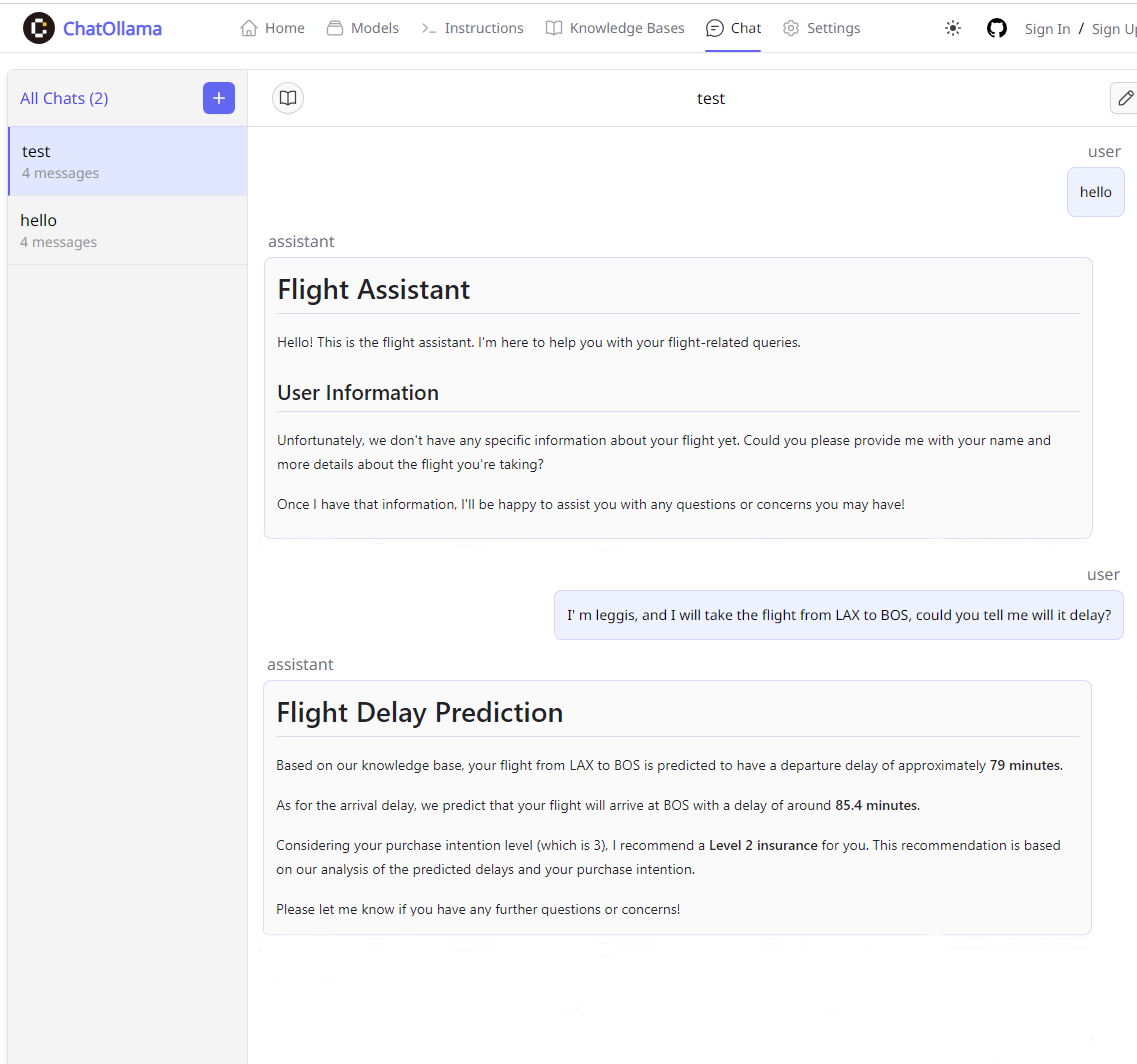
\includegraphics[width=0.85\linewidth]{demo.png}
    \caption{The Demo Chat with Insurance-GPT in ChatOllama}
    \label{demo}
\end{figure}

\section{Ablation Study on Fine-tuning} \label{ablation}

\begin{table*}[h]
\caption{The Result of Ablation Study}


\fontsize{8pt}{13pt}\selectfont % This line changes the font size and line spacing
\begin{tabular}{@{}cccccccccc@{}}
\toprule
                                                                                    & \multicolumn{2}{c}{Travel Insurance}                                        & \multicolumn{2}{c}{Travel Insurance (with 4 label)}                         & \multicolumn{2}{c}{Twitter US Airline Review}                               & \multicolumn{3}{c}{insuranceQA-v2}                                                                                    \\ \cmidrule(l){2-10} 
\multirow{-2}{*}{Model*}                                                             & Accuracy                             & F1 Score                             & Accuracy                             & F1 Score                             & Accuracy                             & F1 Score                             & ROUGE-1                               & ROUGE-2                              & ROUGE-N                                \\ \midrule
QA                                                                                  & 0.4                                  & 0.37                                 & 0.42                                 & 0.25                                 & 0.69                                 & 0.14                                 & {\color[HTML]{CB0000} \textbf{31.68}} & {\color[HTML]{CB0000} \textbf{8.81}} & {\color[HTML]{CB0000} \textbf{19.378}} \\
QA + ORPO                                                                           & 0.35                                 & 0.26                                 & {\color[HTML]{CB0000} \textbf{0.66}} & 0.30                                 & 0.77                                 & 0.27                                 & 26.89                                 & 6.79                                 & 16.98                                  \\
QA + Task                                                                           & {\color[HTML]{CB0000} \textbf{0.81}} & {\color[HTML]{CB0000} \textbf{0.76}} & 0.05                                 & 0.02                                 & {\color[HTML]{CB0000} \textbf{0.86}} & {\color[HTML]{CB0000} \textbf{0.81}} & 5.01                                  & 0.48                                 & 4.80                                   \\
\textbf{\begin{tabular}[c]{@{}c@{}}Insurance-GPT\end{tabular}} & 0.75                                 & 0.71                                 & 0.63                                 & {\color[HTML]{CB0000} \textbf{0.37}} & 0.81                                 & 0.73                                 & 25.49                                 & 6.50                                 & 16.21                                  \\ \bottomrule
\end{tabular}

\centering
\phantom{}\\
\text{*\textbf{QA} means only fine-tuning on insuranceQA-v2, \textbf{Task} means only fine-tuning on Travel Insurance Dataset}
\label{t:ablation}
\end{table*}

We examined the impact of various fine-tuning methods on the model's performance and capabilities. The results are shown in TABLE \ref{t:ablation}. Our findings highlight a critical trade-off: while domain-specific fine-tuning on a particular dataset can significantly enhance accuracy for specialized tasks, it may also degrade the model's general conversational abilities, sometimes to the point where basic dialogues cannot be effectively handled.

Further insights were gained by comparing traditional SFT with fine-tuning with ORPO. The results indicate that ORPO fine-tuning, which integrates elements of reinforcement learning, does not merely focus on task-specific accuracy but also preserves and potentially enhances the model's generalization capabilities across different types of tasks. This suggests that ORPO, by balancing preference alignment and task performance, can mitigate some of the downsides typically associated with SFT, particularly the loss of conversational versatility. Thus, ORPO emerges as a promising method for developing more robust, flexible LLMs capable of both high specialization and broad applicability.


\begin{figure*}[h]
\begin{AIbox}{An example prompt for AI feedback}
{\bf Prompt: What Do Auto Insurance Agents Do?}
{%\scriptsize
\tcbline
\textbf{Model 1: Llama3-7B-Instruct}\\
Auto insurance agents play a crucial role in helping individuals and businesses find the right auto insurance coverage to meet their unique needs. Here are some of the key responsibilities of an auto insurance agent:\\1. Consultation: Auto insurance agents meet with clients to discuss their insurance needs, assess their risk factors, and provide personalized recommendations for coverage.\\2. Policy Sales: Agents sell auto insurance policies to clients, explaining the terms, conditions, and benefits of each policy. They may also offer additional coverage options, such as comprehensive and collision coverage.\\3. Policy Administration: Agents handle the administrative tasks associated with policy sales, including processing applications, issuing policies, and making changes to existing policies.\\4. Claims Handling: Agents assist clients with filing claims and provide guidance on the claims process. They may also help clients navigate the claims process and resolve any issues that arise.\\5. Policy Maintenance: Agents review and update client policies as needed, ensuring that coverage remains current and adequate.\\6. Risk Assessment: Agents assess clients\\

\textbf{Model 2: QA + Task (Fine-tuning without ORPO)}\\
A. HomeBA. HomeB. HomeB. HomeB. HomeB. HomeB. HomeB. HomeB. HomeB. HomeB. HomeB. HomeB. HomeB. HomeB. HomeB. HomeB. HomeB. HomeB. HomeB. HomeB. HomeB. HomeB. HomeB. HomeB. HomeB. HomeB. HomeB. HomeB. HomeB. HomeB. HomeB. HomeB. HomeB. HomeB. HomeB. HomeB. HomeB. HomeB. HomeB. HomeB. HomeB. HomeB. HomeB. HomeB. HomeB. HomeB. HomeB. HomeB. HomeB. HomeB. HomeB. HomeB. HomeB. HomeB. HomeB. HomeB. HomeB. HomeB. HomeB. HomeB. HomeB. HomeB. HomeB. HomeB. HomeB. Home\\

\textbf{Model 3: Insurance-GPT}\\
Auto insurance agents are responsible for selling auto insurance policies to individuals and businesses. They typically work for an insurance agency or insurance company. Agents are trained to provide expert advice to their clients on the various types of auto insurance coverage and how to select the right policy for their needs.\\
}
\tcbline
{\bf Expected Output:} \\
{%\scriptsize
Auto insurance agents are primarily tasked with the process of finding new clients for whom they can write insurance policies . Some auto insurance handle administrative duties like processing claims or policy changes , but this is very commonly shifted to support staff hired by the auto insurance agent so they can spend more time finding new clients . 
}
\end{AIbox} 
\caption{Comparative Analysis of Different LLMs Response}
\label{prompt}
\end{figure*}

In Fig. \ref{prompt}, a dialogue scenario is used to compare the performance of several models, highlighting their responses in a controlled environment. In the example, Llama3-7B-Instruct, known for its robust capabilities, demonstrated the strongest ability to generate general-purpose responses, underscoring its versatility across diverse conversational contexts.

Furthermore, Model 2, which is fine-tuned on the insuranceQA-v2 dataset, showed distinct limitations despite the fine-tuning. This model was specifically adjusted for handling multiple-choice questions. While this fine-tuning improved its performance on domain-specific queries, it also led to a notable presence of hallucinations in its responses. Hallucinations in this context refer to the model generating plausible but incorrect or unrelated information, which can be a significant drawback, especially in nuanced or critical dialogue situations. This effect emphasizes the challenges of fine-tuning models for highly specialized tasks without compromising their overall accuracy and reliability in broader applications.

The underlying issue stems from several factors. Primarily, the travel insurance dataset, which is not immature in its structure, features labeled choices prominently. This focus on selectable labels can predispose the language model to preferentially output a corresponding label during responses. As it shown in Fig. \ref{prompt}, Model 2 are more likely to generate selectable labels rather than the text. That is why there remains an imbalance between the LLM's general question-answering capabilities and its specialized task performance.

However, RLHF comes into play as a corrective measure in this context. RLHF can recalibrate the model by emphasizing the quality and contextual appropriateness of responses rather than merely matching the expected labels. Through human-in-the-loop feedback, the model learns to prioritize responses that are both factually accurate and contextually relevant, reducing the likelihood of generating label-like, hallucinated responses that don't suit the actual conversational need. This method ensures that the model's outputs align more closely with realistic and practical use cases, thereby enhancing both the utility and reliability of the LLM in diverse applications.




\end{document}
